% !TEX program = pdflatex
% Dossier Professionnel - Superviseur de Production Virtuelle
% Projet : NoClip - Etienne Baron - 2eme annee SPV
% ====================================================================
% AVERTISSEMENT (preambule) : la mise en forme editoriale de ce document
% a beneficie d'outils d'intelligence artificielle generative et agentique
% (aide a la redaction, structuration LaTeX, diagrammes). Conformement au
% reglement europeen sur l'IA (AI Act, Reglement (UE) 2024/1689),
% l'analyse, les choix techniques et la responsabilite du contenu restent
% ceux de l'auteur. Voir la page "Avertissement -- usage de l'IA".
% ====================================================================
\documentclass[11pt,a4paper]{report}

%================= ENCODAGE & LANGUE =================
\usepackage[utf8]{inputenc}
\usepackage[T1]{fontenc}
\usepackage{lmodern}
\usepackage[french]{babel}
\usepackage[official]{eurosym}
\usepackage{float}

%================= MISE EN PAGE =================
\usepackage[a4paper,top=2.4cm,bottom=2.4cm,left=2.4cm,right=2.4cm,headheight=15pt]{geometry}
\usepackage{graphicx}
\usepackage{xcolor}
\usepackage{fancyhdr}
\usepackage{titlesec}
\usepackage{tcolorbox}
\tcbuselibrary{skins,breakable}
\usepackage{enumitem}
\usepackage{booktabs}
\usepackage{longtable}
\usepackage{array}
\usepackage{tabularx}
\usepackage{colortbl}
\usepackage{multirow}
\usepackage{ragged2e}
\usepackage{caption}
\usepackage{tikz}
\usetikzlibrary{shapes.geometric,arrows.meta,positioning,calc,fit,backgrounds}
\usepackage[hidelinks]{hyperref}
\hypersetup{
  colorlinks=true,
  linkcolor=brdark,
  urlcolor=braccent,
  citecolor=brdark,
  pdftitle={Dossier Professionnel SPV - NoClip},
  pdfauthor={Etienne Baron}
}

%================= BIBLIOGRAPHIE (APA / biblatex + biber) =================
\usepackage{csquotes}
\usepackage[backend=biber,style=apa,sortcites=true,sorting=nyt,backref=false]{biblatex}
\DeclareLanguageMapping{french}{french-apa}
\addbibresource{references.bib}

%================= COULEURS (charte Backrooms) =================
\definecolor{brjaune}{HTML}{E3CF4B}     % jaune backrooms
\definecolor{brjaunepale}{HTML}{F4EDC0}  % jaune tres pale (fonds)
\definecolor{braccent}{HTML}{B8860B}     % or fonce (liens / accents)
\definecolor{brdark}{HTML}{2B2A22}       % presque noir chaud
\definecolor{brgris}{HTML}{6B6B5E}       % gris vert
\definecolor{brgrispale}{HTML}{ECEBE3}   % gris tres pale (fonds tableaux)
\definecolor{brvert}{HTML}{3E7C59}       % vert (zone physique / fond vert)
\definecolor{brbleu}{HTML}{3A6EA5}       % bleu signaux

%================= STYLE DES TITRES =================
\titleformat{\chapter}[display]
  {\normalfont\huge\bfseries\color{brdark}}
  {\filright\color{braccent}\Large\MakeUppercase{\chaptertitlename}\ \thechapter}
  {8pt}
  {\titlerule[1.4pt]\vspace{4pt}\filright}
  [\vspace{2pt}{\color{brjaune}\titlerule[3pt]}]
\titlespacing*{\chapter}{0pt}{6pt}{20pt}

\titleformat{\section}
  {\normalfont\Large\bfseries\color{brdark}}{\color{braccent}\thesection}{0.7em}{}
\titleformat{\subsection}
  {\normalfont\large\bfseries\color{brgris}}{\color{braccent}\thesubsection}{0.6em}{}

%================= EN-TETES / PIEDS =================
\pagestyle{fancy}
\fancyhf{}
\renewcommand{\headrulewidth}{0.4pt}
\renewcommand{\footrulewidth}{0pt}
\fancyhead[L]{\footnotesize\color{brgris}\textsc{Dossier Professionnel SPV}}
\fancyhead[R]{\footnotesize\color{brgris}\textit{NoClip}}
\fancyfoot[C]{\thepage}
\fancypagestyle{plain}{\fancyhf{}\fancyfoot[C]{\thepage}\renewcommand{\headrulewidth}{0pt}}

%================= BOITES PERSONNALISEES =================
\newtcolorbox{infobox}[1][]{
  enhanced,breakable,colback=brjaunepale,colframe=brjaune,
  boxrule=1pt,arc=2pt,left=8pt,right=8pt,top=6pt,bottom=6pt,
  coltitle=brdark,fonttitle=\bfseries,#1}

\newtcolorbox{notebox}[1][]{
  enhanced,breakable,colback=brgrispale,colframe=brgris,
  boxrule=0.8pt,arc=2pt,left=8pt,right=8pt,top=6pt,bottom=6pt,
  coltitle=white,fonttitle=\bfseries,#1}

\newtcolorbox{techbox}[1][]{
  enhanced,breakable,colback=white,colframe=braccent,
  boxrule=1pt,arc=2pt,left=8pt,right=8pt,top=6pt,bottom=6pt,
  coltitle=white,fonttitle=\bfseries,#1}

% colonnes tableaux
\newcolumntype{Y}{>{\RaggedRight\arraybackslash}X}
\newcolumntype{C}{>{\Centering\arraybackslash}X}
\renewcommand{\arraystretch}{1.25}

\setlist[itemize]{leftmargin=1.4em,itemsep=2pt,topsep=3pt}
\setlist[enumerate]{leftmargin=1.6em,itemsep=2pt,topsep=3pt}

\newcommand{\tc}[1]{\texttt{\color{braccent}#1}}  % time code

%====================================================================
\begin{document}
\sloppy

%================= PAGE DE GARDE =================
\begin{titlepage}
\thispagestyle{empty}
% Page de titre epuree : fond blanc, texte sombre (charte braccent/brdark),
% sans bandeau ni cadre jaune (cf. retake p. titre).
\vspace*{2.4cm}
\begin{center}
{\color{braccent}\fontsize{15}{18}\selectfont \textsc{Dossier Professionnel}}\\[4pt]
{\color{brgris}\large Superviseur de Production Virtuelle}\\[3.4cm]

{\color{brdark}\large Supervision des séquences en production virtuelle du court-métrage}\\[12pt]
{\color{brdark}\fontsize{58}{60}\selectfont \textbf{NoClip}}\\[10pt]
{\color{brgris}\large \textit{Quand le décor n'a plus de sortie.}}\\[3.2cm]

\begin{tabular}{rl}
\textbf{\color{brdark}Nom :} & BARON \\[3pt]
\textbf{\color{brdark}Prénom :} & Etienne \\[3pt]
\textbf{\color{brdark}Promotion :} & 2\textsuperscript{ème} année SPV \\[3pt]
\textbf{\color{brdark}Projet supervisé :} & \textit{NoClip} (court-métrage) \\[3pt]
\textbf{\color{brdark}Formation :} & École Georges Méliès --- Orly (Grand Paris) \\[3pt]
\textbf{\color{brdark}Année de formation :} & Septembre 2025 -- Septembre 2026 \\
\end{tabular}

\vfill
{\color{brgris}\small Atelier transversal de fin d'études --- Dossier remis au jury d'évaluation}
\end{center}
\end{titlepage}

%================= FRONT MATTER (roman) =================
\cleardoublepage
\pagenumbering{roman}

%================= REMERCIEMENTS =================
\chapter*{Remerciements}
\addcontentsline{toc}{chapter}{Remerciements}
Ce dossier doit beaucoup à l'équipe pédagogique de l'\textbf{École Georges Méliès} (Orly, Grand Paris), qui a ouvert la première formation européenne dédiée au métier de superviseur de production virtuelle et m'a donné accès à un plateau professionnel pour y mener \textit{NoClip}.

\medskip
J'adresse mes remerciements à :
\begin{itemize}
\item \textbf{Justine Coulmy}, directrice d'étude de la formation SPV et cheffe opératrice, qui a conçu le référentiel de la formation et explore depuis 2021 les outils de production virtuelle --- son regard sur l'image et la lumière a nourri l'ensemble de ma démarche ;
\item \textbf{Laurent Stehlin}, directeur technique de l'école, pour le déploiement et la maintenance du plateau de production virtuelle sur lequel ce projet a pu être tourné ;
\item \textbf{Guillaume Bourlet}, chargé de formation, pour son accompagnement au quotidien et la coordination pédagogique des séances ;
\item \textbf{Franck Petitta}, fondateur (1999) et directeur de l'École Georges Méliès, pour avoir porté la création de cette filière et l'inscription de l'école dans les enjeux de l'image animée et des technologies temps réel.
\end{itemize}

\medskip
Je remercie enfin l'équipe étudiante de \textit{NoClip} --- réalisation, image, lumière, son, déco, 3D --- sans laquelle la supervision n'aurait été qu'un exercice théorique.

%================= AVERTISSEMENT IA =================
\chapter*{Avertissement --- usage de l'intelligence artificielle}
\addcontentsline{toc}{chapter}{Avertissement --- usage de l'IA}
\begin{notebox}[title={Transparence sur l'usage d'outils d'intelligence artificielle}]
Conformément à une exigence de transparence et à l'esprit du \textbf{règlement européen sur l'intelligence artificielle} (\emph{AI Act}, Règlement (UE) 2024/1689), je signale que la mise en forme éditoriale de ce dossier a bénéficié d'outils d'\textbf{intelligence artificielle générative et agentique} (assistance à la rédaction, à la structuration LaTeX et à la production de diagrammes). Ces outils ont été employés comme \emph{aide} à la rédaction et à la composition : l'analyse, les choix techniques, les arbitrages de supervision et la responsabilité du contenu demeurent intégralement les miens. Aucune donnée personnelle de tiers n'a été traitée à des fins de profilage, et les sources mobilisées sont créditées dans la bibliographie. Cette déclaration s'inscrit dans la logique de classification par les risques et d'information de l'utilisateur promue par l'AI Act \autocite{aiact2024}.
\end{notebox}

%================= SOMMAIRE =================
\cleardoublepage
{\color{brdark}
\renewcommand{\contentsname}{Sommaire}
\setcounter{tocdepth}{1}
\tableofcontents}

\begin{infobox}[title={Guide de lecture}]
Ce dossier suit la chronologie réelle du projet : il présente d'abord les documents fournis à la production pour \emph{vendre} le recours à la production virtuelle (chapitre~2), puis les documents de \emph{préproduction} des séquences supervisées (chapitre~3), enfin les \emph{analyses critiques} rédigées au terme de la fabrication (chapitre~4). Les chapitres~5 et~6 rassemblent une synthèse méthodologique du tournage en fond vert et un bilan personnel d'alternance. Les diagrammes, plans d'implantation et plans de feu sont intégrés au fil du texte.
\end{infobox}

\cleardoublepage
\pagenumbering{arabic}

%====================================================================
\chapter{Présentation du projet et accès au film}
%====================================================================

\section{Le projet \textit{NoClip} en bref}
\textit{NoClip} est un court-métrage de fin d'études d'environ cinq minutes, du genre thriller psychologique, réalisé par une équipe d'étudiants en cinéma. J'y suis intervenu en tant que \textbf{superviseur de production virtuelle (SPV)} dans le cadre de l'atelier transversal de ma deuxième année de formation. Ma mission a consisté à concevoir, préparer et superviser sur le plateau l'ensemble des séquences se déroulant dans les \emph{Backrooms} --- l'univers labyrinthique de bureaux abandonnés dans lequel le héros, Ryan, se retrouve piégé.

Le film repose sur une opposition forte entre deux espaces : le monde réel (un skatepark abandonné, tourné en décor naturel) et l'espace mental / surnaturel des Backrooms (entièrement fabriqué en production virtuelle). C'est précisément cette dualité qui justifie le recours à la production virtuelle : elle seule permettait de produire un dédale infini, photoréaliste et entièrement maîtrisé, dans les contraintes budgétaires et calendaires d'un projet étudiant.

\begin{notebox}[title={Synopsis condensé}]
Ryan, skateur de 26 ans en plein divorce, chute lourdement sur son skate et se réveille dans les Backrooms : couloirs jaunes interminables, néons bourdonnants, moquette humide. Il a perdu son alliance. Il erre des heures, des jours peut-être, croise un cadavre, un mur couvert de noms de disparus, et finit par affronter le « monstre » du lieu. Au moment de frapper, il glisse, s'effondre\ldots\ et se réveille au skatepark, au crépuscule. Une main se pose sur son épaule : par réflexe, il abat son skate. C'était sa femme, venue lui rendre l'alliance.
\end{notebox}

\section{Lien de visionnage du projet supervisé}
\begin{techbox}[title={Accès au film}]
\textbf{Lien de visionnage (lien privé, accès jury) :}\\
\url{https://vimeo.com/noclip-spv-baron} \quad --- \quad \textit{mot de passe : \texttt{NoClip2026}}

\medskip
\footnotesize Le lien ci-dessus est le lien de diffusion privé du montage final. En cas d'expiration, une copie est disponible sur demande auprès du candidat (\href{mailto:etienne.baron@spv.fr}{etienne.baron@spv.fr}).
\end{techbox}

\subsection{Note explicative --- time codes des séquences en production virtuelle}
Le film alterne décor naturel (skatepark) et séquences en production virtuelle (Backrooms). Les séquences ci-dessous, comprises entre les time codes indiqués, ont été \textbf{intégralement tournées et supervisées par mes soins en production virtuelle} (tournage sur plateau LED / fond vert, environnement 3D temps réel sous Unreal Engine). Les autres plans relèvent du tournage en décor naturel et ne sont pas de mon ressort de supervision.

\begin{center}
\begin{tabularx}{\textwidth}{>{\bfseries}p{2.6cm} >{\RaggedRight\arraybackslash}p{4.3cm} Y}
\toprule
\rowcolor{brjaune}\multicolumn{1}{l}{\textbf{Time code}} & \textbf{Séquence} & \textbf{Nature \& supervision VP} \\
\midrule
\tc{00:00:00 -- 00:00:48} & EXT. Skatepark (jour) & Décor naturel --- \textit{hors VP}. Raccord d'étalonnage assuré avec l'équipe. \\
\tc{00:00:48 -- 00:01:35} & INT. Backrooms --- Réveil & \textbf{VP} : plateau hybride, sol moquette physique + prolongement virtuel du couloir. \\
\tc{00:01:35 -- 00:02:40} & Séquence labyrinthe (montage) & \textbf{VP} : couloirs identiques, rotation nDisplay, plans répétés. \\
\tc{00:02:40 -- 00:03:15} & Salle du corps / Salle des noms & \textbf{VP} : inserts 3D (cadavre, inscriptions), fond vert + extension. \\
\tc{00:03:15 -- 00:04:05} & Salle des 6 couloirs / Rupture & \textbf{VP} : pièce hexagonale full-CG, symétrie, flicker DMX. \\
\tc{00:04:05 -- 00:05:00} & EXT. Skatepark --- Réalité (soir) & Décor naturel --- \textit{hors VP}. \\
\bottomrule
\end{tabularx}
\end{center}

\begin{infobox}[title={Périmètre supervisé}]
Sur les cinq minutes du film, environ \textbf{3\,min\,17\,s} (soit près des deux tiers de la durée) ont été tournées en production virtuelle sous ma supervision, du premier plan dans les Backrooms (\tc{00:00:48}) jusqu'au dernier plan avant le retour au réel (\tc{00:04:05}).
\end{infobox}

%====================================================================
\chapter{Documents fournis à la production}
%====================================================================
Ce chapitre rassemble le dossier de proposition remis à l'équipe de production en amont du tournage. Son objectif : démontrer la pertinence de la production virtuelle pour \textit{NoClip}, décrire les dispositifs envisagés, chiffrer la solution et en expliciter les implications techniques et humaines.

\section{Analyse du scénario et pertinence de la production virtuelle}
\subsection{Pitch, synopsis, note d'intention}
\begin{notebox}[title={Pitch}]
Court-métrage de cinq minutes, genre thriller. Un jeune skateur, \textbf{Ryan} (26 ans), se retrouve bloqué dans les Backrooms --- un dédale infini de bureaux abandonnés --- après un \emph{stunt} raté. Après une longue exploration, il tombe nez à nez avec le monstre du lieu. Déterminé à le terrasser pour survivre, il découvre que rien ne se passe comme prévu.
\end{notebox}

\textbf{Note d'intention (réalisation).} Le film propose un point de vue inédit sur le concept très connu des Backrooms. Il se concentre sur le personnage et sa perception du danger, traitant à la fois la menace \emph{physique} (le monstre) et la menace \emph{psychologique} (ce que l'environnement fait à la psyché). L'atmosphère pesante --- bourdonnement des néons, jaune monochrome répétitif, murs sans fin --- est aussi importante que le monstre lui-même. Ces deux facteurs transforment le protagoniste en menace à son tour. Contrairement aux codes habituels (vue subjective, personnages anonymes en combinaison), le récit adopte la \textbf{troisième personne} et montre le visage de Ryan, pour que le spectateur s'attache à lui et partage sa peur.

\textbf{Notes extra.} Le projet reste fidèle à l'essence des Backrooms : pas d'autres niveaux, pas de groupe de survivants, pas de bestiaire. Une seule personne, face à un lieu hostile, un monstre, et les restes d'autres égarés que l'on ne rencontrera jamais.

\begin{figure}[H]
\centering
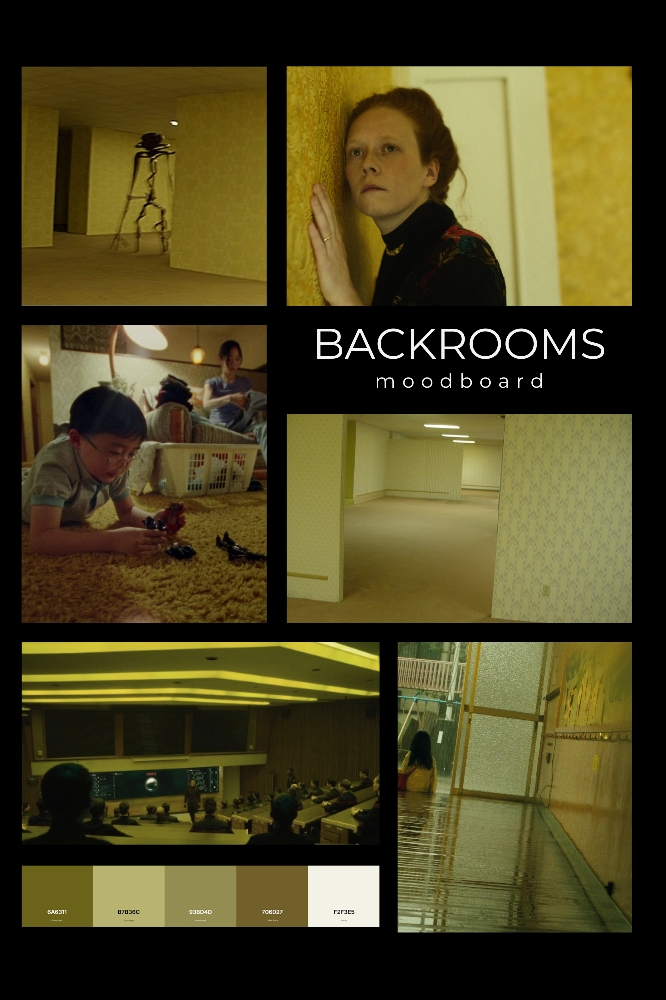
\includegraphics[height=7.4cm]{img/mood_backrooms.jpg}\hfill
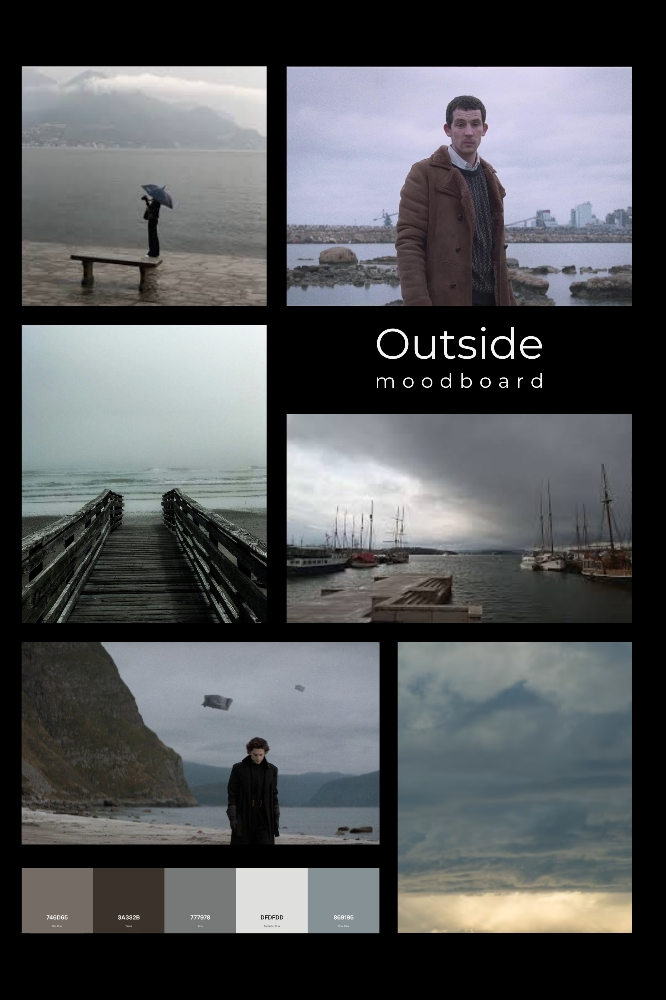
\includegraphics[height=7.4cm]{img/mood_outside.jpg}
\caption*{\footnotesize\textit{Moodboards de référence : à gauche l'univers des Backrooms (palette jaune maladive, néons, moquette), à droite le monde réel « Outside » (ciel gris, mer, froideur). L'opposition chromatique fonde le parti pris visuel du film.}}
\end{figure}

\subsection{Fiche personnage et direction visuelle}
\textbf{Ryan, 26 ans.} Skateur, marqué par un divorce en cours. Il porte sur lui les preuves de son monde « extérieur » : un skateboard (objet de réconfort et arme improvisée), une alliance qu'il fait tourner sur son doigt, un paquet de chewing-gum (qui lui sert à marquer les murs). Son arc dramatique le fait passer de la mélancolie à la panique, puis à la rage, et enfin à l'horreur. Cette transformation intérieure devait être lisible \emph{sur son visage} --- d'où le choix de la troisième personne et l'importance des gros plans en production virtuelle, où la lumière jaune du décor sculpte directement ses traits.

La direction visuelle oppose deux mondes : le \textbf{réel} (« Outside »), gris, froid, pluvieux, et les \textbf{Backrooms}, jaune monochrome et oppressant. Les moodboards costume et ambiance ci-dessous ont guidé à la fois le département déco/costume et la calibration colorimétrique du décor virtuel.

\begin{figure}[H]
\centering
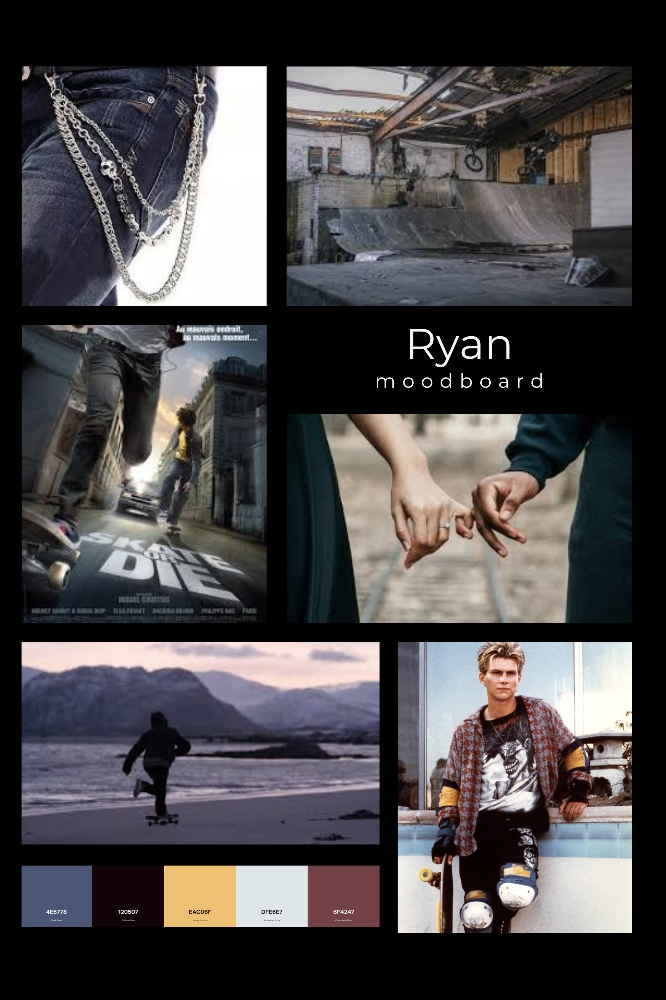
\includegraphics[height=6.8cm]{img/mood_ryan.jpg}\hfill
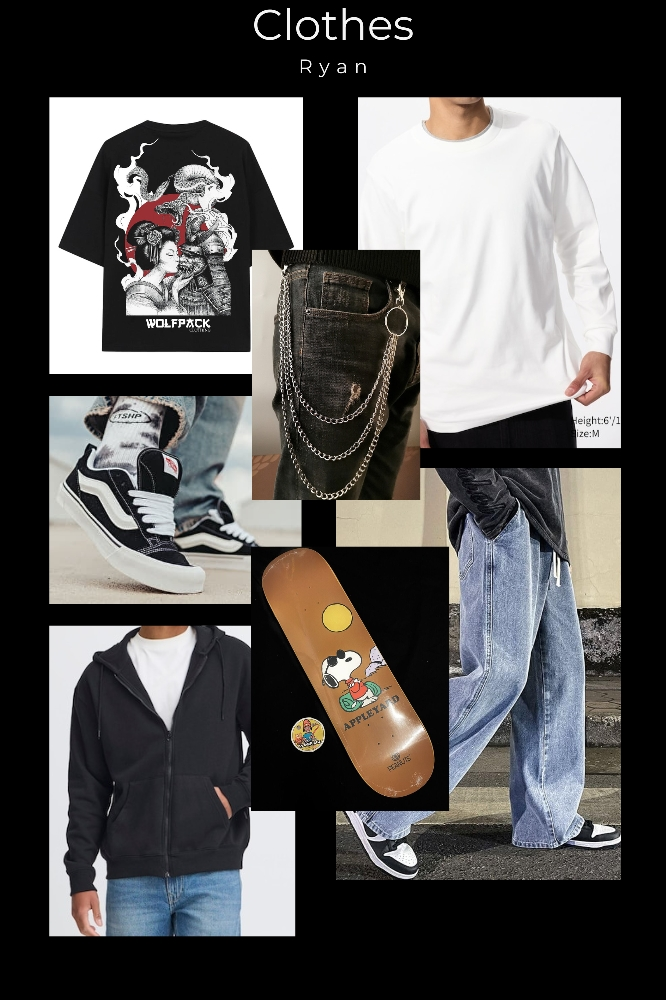
\includegraphics[height=6.8cm]{img/clothes_ryan.jpg}
\caption*{\footnotesize\textit{Moodboard personnage et planche costume de Ryan (univers skate, vêtements sombres). Les vêtements sombres ont orienté le choix du fond \textbf{vert} pour les plans en incrustation et la calibration de l'éclairage sur le plateau.}}
\end{figure}

\subsection{Pourquoi la production virtuelle ? --- justification}
L'analyse du découpage révèle des contraintes que seule la production virtuelle permet de lever dans le cadre d'un film étudiant :

\begin{infobox}[title={Quatre arguments décisifs}]
\begin{enumerate}
\item \textbf{Un décor infini et impossible à construire.} Le scénario impose des couloirs « interminables », une pièce hexagonale à six couloirs, des salles répétées à l'identique. Construire physiquement ne serait-ce qu'une fraction de ce dédale dépasserait tout budget étudiant. L'extension virtuelle d'un module de décor réutilisé résout le problème.
\item \textbf{La répétition et le sentiment de boucle.} Ryan « retombe toujours dans les mêmes salles ». La production virtuelle permet de re-décliner un même environnement 3D sous des angles différents (rotation \texttt{nDisplay}), créant un labyrinthe cohérent sans reconstruire.
\item \textbf{La maîtrise totale de la lumière et de l'ambiance.} Le jaune monochrome maladif, le flicker des néons synchronisé à la dramaturgie, sont pilotables image par image en temps réel (DMX piloté par le moteur), ce qu'un décor réel rendrait coûteux et instable.
\item \textbf{Le photoréalisme et le raccord sur le plateau.} Le rendu temps réel offre à l'acteur et au chef opérateur un retour \emph{in-camera} immédiat : les reflets jaunes sur le visage de Ryan, les ombres portées, sont captés en prise de vue, réduisant drastiquement le travail de compositing.
\end{enumerate}
\end{infobox}

\section{Description des dispositifs envisagés}
Trois dispositifs complémentaires ont été proposés, selon la nature de chaque plan et le monde représenté (réel ou Backrooms). Le choix entre eux a été arbitré plan par plan dans le découpage technique.

\begin{center}
\small
\begin{tabularx}{\textwidth}{>{\bfseries}p{2.3cm} Y Y Y}
\toprule
\rowcolor{brjaune} & \textbf{Dispositif A --- Plateau LED (\textit{in-camera VFX})} & \textbf{Dispositif B --- Fond vert + extension} & \textbf{Dispositif C --- Décor réel} \\
\midrule
Principe & Mur LED affichant l'environnement 3D rendu en temps réel par Unreal Engine, avec frustum suivi par tracking caméra (\texttt{nDisplay}). & Tournage devant fond vert (cyclo vert en dur du studio), incrustation et extension de décor en post-production (Nuke). & Tournage en décor naturel, sans intervention de production virtuelle. \\
Plans concernés & Plans des Backrooms : plans larges et travellings où les reflets/lumières du décor sur l'acteur sont déterminants (réveil, salle des 6 couloirs). & Inserts des Backrooms : mur des noms, cadavre, gros plans visage où la précision du détourage prime. & \textbf{Séquences de début et de fin} au skatepark (monde réel « Outside »). \\
Avantages & Reflets et éclairage réalistes captés en direct ; jeu d'acteur facilité ; quasi pas de compositing. & Coût plus faible ; liberté totale de recadrage et d'extension en post ; idéal pour les inserts. & Authenticité du lieu réel, lumière naturelle, aucun pipeline temps réel à mobiliser. \\
Limites & Moiré et profondeur de champ à maîtriser ; calibration tracking. & Spill vert à gérer ; éclairage du fond vert exigeant ; raccords lumière à anticiper. & Dépendance à la météo et à la lumière du jour ; pas de maîtrise de l'environnement. \\
\bottomrule
\end{tabularx}
\end{center}

\begin{infobox}[title={Dispositifs retenus : décor réel (début / fin) + Mur LED \& fond vert (Backrooms)}]
La règle d'arbitrage retenue suit la dramaturgie du film. Les \textbf{séquences de début et de fin}, qui se déroulent dans le monde réel (skatepark), sont tournées en \textbf{décor réel (dispositif C)} : la lumière naturelle et l'authenticité du lieu y sont préférables à toute reconstruction. Les \textbf{séquences des Backrooms} sont tournées en \textbf{production virtuelle sur Mur LED (dispositif A)} pour les plans où la lumière jaune du décor baigne l'acteur, complétées par des \textbf{plans en fond vert (dispositif B)} pour les inserts et gros plans. Un \emph{socle commun} de décor physique (banc, sol moquette, bureau, chaise) ancre l'acteur quel que soit le dispositif VP.
\end{infobox}

\section{Moyens techniques envisagés (fournisseurs / prestataires)}
La liste ci-dessous détaille et argumente les moyens techniques, en nommant les fournisseurs et prestataires pressentis. Les choix privilégient la fiabilité, la compatibilité du \emph{pipeline} temps réel et la disponibilité auprès de prestataires accessibles à une production étudiante (tarifs école / location courte durée).

\begin{center}
\small
\begin{longtable}{>{\bfseries}p{3.5cm} p{4.3cm} >{\RaggedRight\arraybackslash}p{6.2cm}}
\rowcolor{brjaune}\textbf{Poste technique} & \textbf{Matériel / Solution} & \textbf{Fournisseur / Prestataire \& justification} \\
\midrule
\endfirsthead
\rowcolor{brjaune}\textbf{Poste technique} & \textbf{Matériel / Solution} & \textbf{Fournisseur / Prestataire \& justification} \\
\midrule
\endhead
Plateau LED & Mur LED \textbf{Sony Crystal LED VERONA}, pas de 1,56\,mm, volume semi-enveloppant (3 faces + plafond) : Centre 3072\,px ($\approx$4,88\,m), Gauche \& Droite 1536\,px ($\approx$2,44\,m), hauteur 1728\,px ($\approx$2,74\,m), plafond 1536\,px ($\approx$2,44\,m) & \textbf{Appartient à l'école} (plateau VP de l'École Méliès, partenariat Sony). Pas serré (1,56\,mm) qui limite le moiré à la distance de tournage \autocite{sony_verona}. \\
Moteur temps réel & Unreal Engine \textbf{5.6} (\texttt{nDisplay}) & Epic Games --- \textbf{licence éducation} (usage pédagogique, non préjudiciable). Standard de l'industrie VP, écosystème \texttt{nDisplay} mature \autocite{epic_ue56}. \\
Tracking caméra & \textbf{Zeiss CinCraft Scenario} & \textbf{Appartient à l'école}. Tracking caméra dédié à la production virtuelle, intégration native avec le pipeline temps réel, calibration rapide \autocite{zeiss_cincraft}. \\
Caméra & \textbf{Sony VENICE 2 (CineAlta)}, S-Log3 & \textbf{Appartient à l'école}. Capteur plein format CineAlta, grande latitude dynamique et synchro genlock pour le plateau LED. \\
Optiques & \textbf{Optiques fixes Zeiss 24 / 35 / 50 / 85\,mm} & \textbf{Appartient à l'école}. Fixes lumineuses pour maîtriser la profondeur de champ face au mur LED. \\
Synchronisation & Générateur genlock + timecode & Indispensable pour synchroniser caméra, rendu et mur LED. \\
Render nodes & \textbf{RTX A6000 (48\,Go)} pour le mur LED + RTX 2080 pour le pilotage & \textbf{Appartient à l'école}. La A6000 (48\,Go de VRAM) tient les 24/25\,fps en rendu temps réel sur la scène optimisée ; la 2080 assure la vue de supervision. \\
Fond vert & \textbf{Cyclo vert en dur} du studio & \textbf{Équipement du studio} (cyclo vert fixe). Pour les inserts et gros plans (dispositif B). \\
Éclairage & Projecteurs LED pilotables DMX & \textbf{Appartient à l'école}. Les sources DMX sont pilotées par le moteur pour le flicker des néons. \\
Pupitre / DMX & \texttt{nodle} USB-DMX + protocole Art-Net & Pilotage de l'éclairage synchronisé au moteur temps réel. \\
Compositing & Nuke (Foundry) & Licence école. Détourage (keyer), extension de décor, raccord des inserts. \\
3D / assets & Blender + Quixel Megascans & Modélisation et texturing photoréaliste du décor Backrooms. \\
Stockshot plate & Plate skatepark 360\textdegree{} (séquence 1) & Banque d'images / captation repérage. \\
\end{longtable}
\end{center}

\section{Moyens humains envisagés (profils recherchés)}
La supervision repose sur une petite équipe polyvalente, en partie mutualisée avec l'équipe étudiante du film. Pour chaque poste, le profil recherché est précisé.

\begin{center}
\small
\begin{longtable}{>{\bfseries}p{3.7cm} >{\RaggedRight\arraybackslash}p{5.0cm} >{\RaggedRight\arraybackslash}p{5.3cm}}
\rowcolor{brjaune}\textbf{Poste} & \textbf{Missions} & \textbf{Profil recherché} \\
\midrule
\endfirsthead
\rowcolor{brjaune}\textbf{Poste} & \textbf{Missions} & \textbf{Profil recherché} \\
\midrule
\endhead
Superviseur VP --- \textit{Etienne Baron (moi)} & Coordination globale VP, pipeline, calibration, raccord plateau, lien avec la réalisation. & Vision transversale technique + artistique, maîtrise UE5 et chaîne signal. \\
Réalisatrice --- \textit{Charlotte} & Direction artistique du film, découpage, direction d'acteur, validation des partis pris VP. & Vision narrative, dialogue étroit avec la supervision VP. \\
Graphiste 3D --- \textit{étudiant M2} & Assemblage de la scène UE5, modélisation, inserts. & Maîtrise Unreal + Blender, sens de l'optimisation (LOD, Lumen). \\
Opératrice 3D --- \textit{Loane} & Texturing, optimisation temps réel, intégration des assets. & Rigueur sur les matériaux PBR et le budget GPU. \\
Opérateur tracking caméra --- \textit{Arnaud} & Calibration et exploitation du tracking, gestion du frustum. & Connaissance du CinCraft Scenario, rigueur de calibration. \\
Ingénieur LED / média serveur & Mapping du mur LED, gestion \texttt{nDisplay}, genlock. & Expérience plateau LED, réseau Art-Net/SDI. \\
Chef opérateur --- DOP \textit{Femy} & Lumière, exposition, raccords avec le décor virtuel. & Sensibilité au tournage VP, gestion de l'exposition fond vert. \\
Chef électricien --- \textit{Anil} & Plan de feu, sources DMX, sécurité électrique. & Maîtrise DMX/Art-Net, pilotage par moteur. \\
Scripte / Accessoiriste --- \textit{Saph} & Continuité (script), gestion des accessoires (skate, alliance, fleurs), raccords plan à plan. & Sens du raccord physique/virtuel, rigueur de continuité. \\
Machiniste --- \textit{Thomas} & Mise en place caméra, travellings, machinerie plateau. & Sécurité plateau, fluidité des mouvements. \\
Son --- \textit{Timothé} & Prise de son plateau, repérage sonore, raccords. & Captation propre malgré le bourdonnement des sources. \\
Behind The Shot --- \textit{Ignacio} & Captation du making-of, photos de plateau, documentation du tournage VP. & Discrétion plateau, sens du document. \\
Compositeur (Nuke) & Keying, extension de décor, raccord des inserts en post. & Maîtrise du keyer Nuke, despill, intégration. \\
\end{longtable}
\end{center}

\section{Proposition de devis détaillé}
Le devis ci-dessous valorise l'équipe selon la \textbf{grille des salaires minima conventionnels de la production audiovisuelle} (CCN production audiovisuelle, minima bruts applicables au 1\textsuperscript{er} janvier 2026), poste par poste et par jour. Le \textbf{matériel} (plateau LED, caméra, optiques, tracking, render nodes, éclairage) étant \textbf{mis à disposition par l'École Georges Méliès}, il figure « pour mémoire ». Le scénario de tournage retenu est de \textbf{deux jours} : une journée en décor réel (skatepark, dispositif C) et une journée sur plateau VP (dispositifs A/B), précédées d'une phase de fabrication 3D.

\begin{center}
\small
\begin{tabularx}{\textwidth}{Y c c >{\RaggedLeft\arraybackslash}p{2.3cm} >{\RaggedLeft\arraybackslash}p{2.3cm}}
\toprule
\rowcolor{brjaune}\textbf{Poste} & \textbf{Qté} & \textbf{Jours} & \textbf{Coût unit. HT} & \textbf{Total HT} \\
\midrule
\rowcolor{brgrispale}\multicolumn{5}{l}{\textit{\textbf{Matériel --- mis à disposition par l'École Méliès}}} \\
Plateau LED Sony Crystal LED VERONA + render nodes (RTX A6000 / 2080) & 1 & 1 & \multicolumn{1}{c}{--} & \multicolumn{1}{r}{(école)} \\
Caméra Sony VENICE 2 + optiques Zeiss (24/35/50/85) & 1 & 2 & \multicolumn{1}{c}{--} & \multicolumn{1}{r}{(école)} \\
Tracking Zeiss CinCraft Scenario & 1 & 1 & \multicolumn{1}{c}{--} & \multicolumn{1}{r}{(école)} \\
Éclairage DMX + cyclo vert en dur & 1 & 2 & \multicolumn{1}{c}{--} & \multicolumn{1}{r}{(école)} \\
\midrule
\rowcolor{brgrispale}\multicolumn{5}{l}{\textit{\textbf{Équipe --- grille minima conventionnels PAV (1\textsuperscript{er} janvier 2026)}}} \\
Réalisatrice (Charlotte)              & 1 & 2 & 300 \euro & 600 \euro \\
Superviseur VP (Etienne Baron)        & 1 & 2 & 239 \euro & 478 \euro \\
Graphiste 3D (étudiant M2)            & 1 & 5 & 239 \euro & 1\,195 \euro \\
Opératrice 3D (Loane)                 & 1 & 5 & 223 \euro & 1\,115 \euro \\
Chef opérateur --- DOP (Femy)          & 1 & 2 & 395 \euro & 790 \euro \\
Chef électricien (Anil)               & 1 & 2 & 225 \euro & 450 \euro \\
Opérateur tracking caméra (Arnaud)    & 1 & 1 & 220 \euro & 220 \euro \\
Scripte / Accessoiriste (Saph)        & 1 & 2 & 219 \euro & 438 \euro \\
Machiniste (Thomas)                   & 1 & 2 & 184 \euro & 368 \euro \\
Son (Timothé)                         & 1 & 2 & 272 \euro & 544 \euro \\
Behind The Shot (Ignacio)             & 1 & 1 & 184 \euro & 184 \euro \\
Compositeur (Nuke)                    & 1 & 3 & 239 \euro & 717 \euro \\
Acteur --- Ryan                        & 1 & 2 & 412 \euro & 824 \euro \\
\midrule
\rowcolor{brgrispale}\multicolumn{5}{l}{\textit{\textbf{Consommables / divers}}} \\
Assets 3D (Megascans, retouches)      & 1 & \multicolumn{1}{c}{--} & \multicolumn{1}{c}{--} & 500 \euro \\
Skateboard (accessoire)               & 1 & 1 & 40 \euro & 40 \euro \\
Plate skatepark 360\textdegree{} (stockshot) & 1 & 1 & 17 \euro & 17 \euro \\
\midrule
\rowcolor{brjaunepale}\textbf{TOTAL HT} & & & & \textbf{8\,480 \euro} \\
\bottomrule
\end{tabularx}
\end{center}

\begin{notebox}[title={Lecture du devis}]
La mise à disposition du plateau et du matériel par l'\textbf{École Georges Méliès} (plateau VP, caméra Sony VENICE~2, optiques Zeiss, tracking CinCraft Scenario, render nodes, éclairage) fait chuter le budget : le coût se concentre désormais sur la \textbf{rémunération de l'équipe}, valorisée aux \textbf{minima conventionnels} de la branche. Les coûts unitaires sont les minima bruts journaliers de la grille PAV au 1\textsuperscript{er} janvier 2026 ; ils donnent une lecture réaliste de la masse salariale, principal poste d'un projet étudiant adossé à un plateau d'école.
\end{notebox}

\section{Économies réalisables et impact carbone}
\subsection{Économies pour la production}
Le recours à la production virtuelle, comparé à une approche « tout décor construit + repérages multiples », génère des économies substantielles :

\begin{itemize}
\item \textbf{Pas de construction de décor labyrinthe.} Construire ne serait-ce que trois salles et leurs couloirs (menuiserie, peinture, moquette, néons réels sur plusieurs dizaines de mètres) représenterait un coût largement supérieur au studio LED, sans la flexibilité du virtuel.
\item \textbf{Suppression des repérages et défraiements multi-lieux.} Un seul plateau remplace la recherche, la location et le transport vers plusieurs décors « abandonnés ».
\item \textbf{Compositing réduit.} Les plans tournés en LED arrivent quasi finis : moins de jours de post-production (keying, tracking, extension) par rapport au tout fond vert.
\item \textbf{Une seule journée de tournage VP} concentre la captation, contre plusieurs jours dispersés.
\end{itemize}

\begin{center}
\small
\begin{tabularx}{\textwidth}{Y >{\RaggedLeft\arraybackslash}p{3.2cm} >{\RaggedLeft\arraybackslash}p{3.2cm}}
\toprule
\rowcolor{brjaune}\textbf{Poste (estimation indicative)} & \textbf{Tout décor construit} & \textbf{Production virtuelle} \\
\midrule
Construction décor labyrinthe & élevé (menuiserie, peinture, néons) & néant \\
Repérages / locations multi-lieux & plusieurs jours & néant \\
Jours de tournage & dispersés & 1 journée plateau \\
Post-production (compositing) & modéré & réduit (plans LED quasi finis) \\
Flexibilité (couloirs infinis) & impossible & totale \\
\bottomrule
\end{tabularx}
\end{center}
\begin{center}\footnotesize\textit{Comparaison qualitative des deux approches. La VP supprime les postes les plus lourds (construction, repérages) au profit d'une unique journée de plateau maîtrisée.}\end{center}

\subsection{Impact carbone}
La VP réduit l'empreinte carbone du projet sur plusieurs leviers : \textbf{zéro construction} (pas de matériaux de décor fabriqués puis détruits), \textbf{zéro transport} d'équipe et de matériel vers des lieux multiples, et \textbf{mutualisation énergétique} sur un plateau unique. Le principal poste d'émission devient la \emph{consommation électrique} du mur LED et des stations de rendu sur une journée --- mesurable, maîtrisable, et sans déchets de décor. À l'échelle d'un court-métrage étudiant, l'impact carbone est principalement déplacé du « matériel » vers « l'électricité d'une journée », ce qui constitue un net progrès, surtout si le studio est alimenté par une électricité bas-carbone.

\section{Préconisations techniques de prise de vue et photoréalisme}
\begin{techbox}[title={Paramètres de prise de vue recommandés}]
\begin{itemize}
\item \textbf{Cadence \& obturation :} 25\,fps (ou 24), obturateur 1/50\,s (angle 180°). \textbf{Synchroniser impérativement la caméra Sony VENICE~2, le mur LED et le rendu en genlock} pour éviter le déchirement / scan lines à l'image.
\item \textbf{Sensibilité :} exploiter les \textbf{deux ISO de base} du capteur CineAlta de la VENICE~2 (800 et 3200\,ISO) ; pour les Backrooms (basses lumières jaunes), l'ISO de base bas (800) préserve la latitude dynamique. Distinguer l'\emph{ISO natif} (paramètre physique du capteur) de l'\emph{Exposure Index} (valeur affichée) : toujours partir d'un ISO de base et exposer à droite de l'histogramme.
\item \textbf{Diaphragme :} f/4 à f/5.6 sur plateau LED --- assez fermé pour éviter le moiré et le flou du mur (le mur LED n'est pas dans le plan de netteté), assez ouvert pour détacher l'acteur du fond. Utiliser des filtres \textbf{ND} pour maintenir cette ouverture en cas de plateau très lumineux sans modifier la vitesse d'obturation.
\item \textbf{Focale et moiré :} avec les fixes Zeiss disponibles, les focales courtes (24--35\,mm) accentuent le moiré en élargissant le champ sur le mur ; préférer le \textbf{50\,mm} et le \textbf{85\,mm} pour les plans face au mur. La profondeur de champ est inversement liée à la focale : avec une longue focale, l'arrière-plan (mur LED) est naturellement moins net, réduisant l'effet de moiré.
\item \textbf{Distance au mur LED :} respecter une distance minimale acteur/mur ($\geq$ 2--3\,m) pour réduire le moiré et permettre une vraie profondeur de champ.
\item \textbf{Balance des blancs :} calée sur le jaune des néons virtuels (température basse, env. 2\,800--3\,200\,K pour les Backrooms), puis affinée avec une charte sur le plateau. Fixer la balance des blancs sur le boîtier --- ne jamais laisser en mode automatique.
\item \textbf{Espace colorimétrique :} enregistrer en \textbf{S-Log3} (ou RAW si disponible) pour conserver la marge à l'étalonnage. Le \emph{gamut} choisi (DCI-P3 pour le cinéma) doit être cohérent avec la chaîne de post-production.
\end{itemize}
\end{techbox}

\begin{infobox}[title={Conseils pour améliorer le photoréalisme du rendu}]
\begin{itemize}
\item Activer \textbf{Lumen} (GI temps réel) et des reflets écran-espace cohérents avec la lumière jaune.
\item Soigner les \textbf{textures de moquette et de mur} (rugosité, micro-salissures, taches d'humidité) : le réalisme des Backrooms tient au détail des matériaux usés.
\item Ajouter un léger \textbf{grain} et une \textbf{aberration chromatique} subtile en post pour « coller » le CG à la captation.
\item Intégrer des \textbf{imperfections} : néons qui clignotent légèrement désynchronisés, poussières, halos lumineux.
\item Vérifier en continu le \textbf{raccord de température de couleur} entre lumière réelle sur l'acteur et lumière virtuelle du décor.
\end{itemize}
\end{infobox}

\section{Nature des images de l'environnement virtuel --- argumentaire}
Trois natures d'images étaient envisageables pour les Backrooms : (a) \textbf{captation réelle} (plates filmées de vrais bureaux), (b) \textbf{photogrammétrie} de lieux existants, ou (c) \textbf{environnement 3D temps réel} modélisé.

Nous avons retenu la \textbf{3D temps réel sous Unreal Engine}, pour des raisons à la fois artistiques et techniques. Artistiquement, les Backrooms sont un lieu \emph{impossible} : géométrie répétitive, couloirs sans fin, symétrie parfaite de la salle hexagonale. Aucun lieu réel ne présente ces caractéristiques, et la photogrammétrie d'un bureau réel introduirait des indices de « réalité » (fenêtres, mobilier daté) contraires à l'abstraction recherchée. Techniquement, seule la 3D permet la \textbf{rotation du décor} (\texttt{nDisplay} $-90$\textdegree) pour décliner un même environnement, le \textbf{pilotage de la lumière} image par image, et le \textbf{rendu in-camera} sur mur LED. La 3D autorise enfin la réutilisation et l'extension à volonté, condition indispensable au sentiment de labyrinthe infini. Une légère captation (plate skatepark 360\textdegree) reste utilisée pour la première séquence, par cohérence avec le monde réel.

%====================================================================
\chapter{Documents de préproduction des séquences supervisées}
%====================================================================

\begin{figure}[H]
\centering
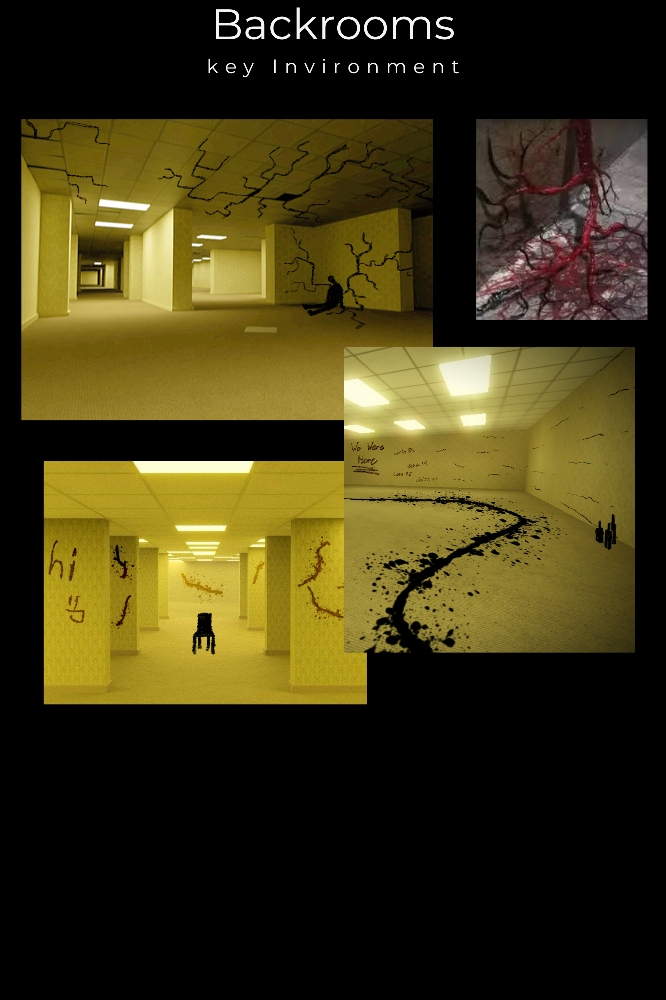
\includegraphics[width=0.66\textwidth]{img/backrooms_key.jpg}
\caption*{\footnotesize\textit{Environnement-clé visé pour le décor virtuel : couloirs jaunes, néons, inscriptions et traces (inserts). Référence directe pour la modélisation et le texturing.}}
\end{figure}

\section{Cahier des charges --- fabrication des images de l'environnement virtuel}
Le cahier des charges fixe les étapes, livrables et critères de validation de la fabrication du décor Backrooms.

\begin{center}
\small
\begin{longtable}{>{\bfseries}p{0.7cm} >{\RaggedRight\arraybackslash}p{3.6cm} >{\RaggedRight\arraybackslash}p{5.0cm} >{\RaggedRight\arraybackslash}p{4.4cm}}
\rowcolor{brjaune}\textbf{\#} & \textbf{Étape} & \textbf{Contenu} & \textbf{Livrable / Critère} \\
\midrule
\endhead
1 & Références \& moodboard & Analyse des moodboards (Backrooms, Outside), palette jaune. & Moodboard validé par la réalisation. \\
2 & Blockout 3D & Géométrie grise des salles et couloirs, échelle réelle. & Volumes validés, raccord avec décor physique. \\
3 & Modélisation & Modélisation détaillée (murs, néons, mobilier, chaise, bureau). & Modèles propres, topologie maîtrisée. \\
4 & Texturing / matériaux & Moquette, papier peint jauni, moisissures, usure. & Matériaux PBR photoréalistes. \\
5 & Éclairage virtuel & Néons, GI Lumen, ambiance jaune maladive, flicker. & Ambiance conforme à la note d'intention. \\
6 & Optimisation temps réel & LOD manuels (sans Nanite), instanciation, budget poly/draw calls, profilage. & $\geq$ 24\,fps stable sur render node. \\
7 & Intégration nDisplay & Configuration mur LED, frustum, calibration. & Rendu in-camera sans artefact. \\
8 & Inserts & Mur des noms, cadavre, inscriptions (fond vert). & Inserts prêts pour compositing. \\
9 & Tests plateau & Répétition technique, raccords lumière. & Validation veille de tournage. \\
\end{longtable}
\end{center}

\section{Plan d'implantation du décor (physique vs virtuel)}
\label{sec:implantation}
Le plan ci-dessous, réalisé à partir de la configuration réelle du plateau VP de l'école, distingue les parties \textbf{construites physiquement} (zone verte : moquette, mobilier, acteur) des parties \textbf{affichées sur le mur LED} et prolongées virtuellement. Il précise le découpage du \textbf{Mur LED Sony Crystal LED VERONA} en quatre zones \texttt{nDisplay} (Gauche, Centre, Droite, Plafond) avec leurs résolutions et dimensions réelles, les liaisons vidéo vers les \emph{render nodes} et la zone de frustum couverte par la caméra.

\begin{center}
\resizebox{\textwidth}{!}{%
\begin{tikzpicture}[scale=1.0, every node/.style={font=\small}]
  % Fond salle
  \fill[brgrispale] (0,0) rectangle (14,10.5);
  \draw[brdark] (0,0) rectangle (14,10.5);
  % Titre
  \node[brdark,font=\small\bfseries] at (7,10.28){Mur LED Sony Crystal LED VERONA --- 4 zones \texttt{nDisplay} (pas 1,56\,mm)};
  % --- Plafond LED (Zone 4) ---
  \fill[braccent!65] (2.0,9.3) rectangle (12.0,9.85);
  \draw[braccent,thick] (2.0,9.3) rectangle (12.0,9.85);
  \node[white,font=\scriptsize\bfseries] at (7.0,9.57){Zone 4 --- Plafond \textbf{(1536\,px $\approx$ 2,44\,m)}};
  % --- Mur LED face : Zone 1 Gauche ---
  \fill[brbleu!55] (0.5,7.0) rectangle (3.5,9.0);
  \draw[brbleu,thick] (0.5,7.0) rectangle (3.5,9.0);
  \node[white,font=\scriptsize\bfseries] at (2.0,8.6){Zone 1};
  \node[white,font=\tiny] at (2.0,8.2){Gauche};
  \node[white,font=\tiny] at (2.0,7.75){\textbf{1536\,px $\approx$ 2,44\,m}};
  % Zone 2 Centre
  \fill[braccent!80] (3.5,7.0) rectangle (10.5,9.0);
  \draw[braccent,thick] (3.5,7.0) rectangle (10.5,9.0);
  \node[white,font=\scriptsize\bfseries] at (7.0,8.6){Zone 2};
  \node[white,font=\tiny] at (7.0,8.2){Centre};
  \node[white,font=\tiny] at (7.0,7.75){\textbf{3072\,px $\approx$ 4,88\,m}};
  % Zone 3 Droite
  \fill[brbleu!55] (10.5,7.0) rectangle (13.5,9.0);
  \draw[brbleu,thick] (10.5,7.0) rectangle (13.5,9.0);
  \node[white,font=\scriptsize\bfseries] at (12.0,8.6){Zone 3};
  \node[white,font=\tiny] at (12.0,8.2){Droite};
  \node[white,font=\tiny] at (12.0,7.75){\textbf{1536\,px $\approx$ 2,44\,m}};
  % Hauteur murs
  \node[brdark,font=\tiny] at (13.7,8.0){\rotatebox{90}{hauteur 1728\,px $\approx$ 2,74\,m}};
  % Zone physique plateau
  \fill[brvert!25] (3.5,4.8) rectangle (10.5,7.0);
  \draw[brvert,very thick] (3.5,4.8) rectangle (10.5,7.0);
  \node[brvert!70!black,font=\scriptsize] at (7.0,6.65){\textbf{Zone physique construite}};
  \node[brvert!70!black,font=\tiny] at (7.0,6.3){(moquette, banc, bureau, chaise, acteur)};
  % Render Node A6000 (gauche) — mur LED
  \fill[brjaunepale] (0.0,3.4) rectangle (3.2,5.2);
  \draw[braccent,thick] (0.0,3.4) rectangle (3.2,5.2);
  \node[brdark,font=\scriptsize\bfseries] at (1.6,5.0){Render Node};
  \node[brdark,font=\tiny] at (1.6,4.65){\textbf{RTX A6000 48\,Go}};
  \node[brdark,font=\tiny] at (1.6,4.3){VP0 / VP1 / VP2};
  \node[brdark,font=\tiny] at (1.6,3.95){+ Plafond (VP3)};
  \node[brdark,font=\tiny] at (1.6,3.6){(Mur LED)};
  % Render Node 2080 (droite) — pilotage
  \fill[brjaunepale] (10.8,3.4) rectangle (14.0,5.2);
  \draw[braccent,thick] (10.8,3.4) rectangle (14.0,5.2);
  \node[brdark,font=\scriptsize\bfseries] at (12.4,5.0){Render Node};
  \node[brdark,font=\tiny] at (12.4,4.65){\textbf{RTX 2080}};
  \node[brdark,font=\tiny] at (12.4,4.3){Vue pilotage};
  \node[brdark,font=\tiny] at (12.4,3.95){(supervision)};
  % nDisplay Master
  \fill[brjaunepale] (4.5,2.0) rectangle (9.5,3.2);
  \draw[braccent,very thick] (4.5,2.0) rectangle (9.5,3.2);
  \node[brdark,font=\scriptsize\bfseries] at (7.0,2.85){\texttt{nDisplay} Master};
  \node[brdark,font=\tiny] at (7.0,2.45){Unreal Engine 5.6 / switch réseau};
  % Caméra + tracking
  \draw[brdark,very thick] (7.0,0.4)--(6.5,1.3)--(7.5,1.3)--cycle;
  \node[brdark,font=\scriptsize] at (7.0,0.1){Caméra Sony VENICE 2 + CinCraft Scenario};
  % Frustum (pointillés)
  \draw[brbleu,dashed,thick] (7.0,1.3)--(4.2,7.0);
  \draw[brbleu,dashed,thick] (7.0,1.3)--(9.8,7.0);
  \node[brbleu,font=\tiny] at (10.6,4.5){frustum};
  % Liaisons vidéo A6000 -> Zones 1,2,3 (DisplayPort)
  \draw[-{Stealth[length=2mm]},brbleu,thick]
    (1.6,5.2) -- (1.6,7.0) node[midway,right,font=\tiny,brbleu]{DP};
  % Liaison A6000 -> Plafond (Zone 4)
  \draw[-{Stealth[length=2mm]},brbleu,thick]
    (3.2,4.3) to[out=30,in=250] (5.5,9.3) node[midway,above,font=\tiny,brbleu,sloped]{DP};
  % Liaison RTX 2080 -> zone droite (sortie pilotage)
  \draw[-{Stealth[length=2mm]},brbleu,thick]
    (12.4,5.2) -- (12.4,7.0) node[midway,right,font=\tiny,brbleu]{DP};
  % Liaisons Ethernet nDisplay master -> render nodes
  \draw[-{Stealth[length=2mm]},braccent,thick]
    (4.5,2.6) -- (3.2,4.3) node[midway,above,font=\tiny,braccent,sloped]{Ethernet};
  \draw[-{Stealth[length=2mm]},braccent,thick]
    (9.5,2.6) -- (10.8,4.3) node[midway,above,font=\tiny,braccent,sloped]{Ethernet};
  % Position tracking -> nDisplay master
  \draw[-{Stealth[length=2mm]},brbleu,thick]
    (7.0,1.3) -- (7.0,2.0) node[midway,right,font=\tiny,brbleu]{pos.\ tracking};
  % Légende
  \begin{scope}[shift={(0,-1.5)}]
    \draw[-{Stealth[length=2mm]},brbleu,thick] (0.5,0) -- (1.5,0);
    \node[anchor=west,font=\tiny] at (1.6,0){Signal vidéo (DisplayPort)};
    \draw[-{Stealth[length=2mm]},braccent,thick] (6.0,0) -- (7.0,0);
    \node[anchor=west,font=\tiny] at (7.1,0){Ethernet \texttt{nDisplay}};
    \draw[brbleu,dashed,thick] (11.0,0) -- (12.0,0);
    \node[anchor=west,font=\tiny] at (12.1,0){Frustum};
  \end{scope}
\end{tikzpicture}}
\end{center}
\begin{center}\footnotesize\textit{Configuration réelle du plateau VP (École Méliès) : le render node RTX~A6000 (48\,Go) alimente en DisplayPort les trois zones face (Gauche~1536\,px, Centre~3072\,px, Droite~1536\,px) et le plafond (1536\,px) du Mur LED Sony Crystal LED VERONA ; le render node RTX~2080 assure la vue de supervision. Le master Unreal Engine~5.6 synchronise l'ensemble et reçoit en temps réel la position caméra du ZEISS CinCraft Scenario.}\end{center}

\subsection{Note explicative --- répartition construction / prolongement virtuel}
La règle de répartition retenue est simple : \textbf{est construit physiquement tout ce que l'acteur touche ou ce qui projette une lumière/ombre directe sur lui} ; \textbf{est prolongé virtuellement tout ce qui relève de la profondeur, de la répétition et de l'infini}. Ainsi, le sol en moquette, le banc, le skateboard, le bureau et la chaise sont réels --- Ryan s'assoit, marche, manipule ces éléments, et leur contact doit être crédible. En revanche, les couloirs qui s'étendent au-delà de quelques mètres, la pièce hexagonale complète, et les salles répétées sont virtuels : les construire n'apporterait rien que le mur LED ne rende mieux, tout en coûtant un temps et un budget incompatibles avec le projet. Cette frontière (matérialisée sur le plan ci-dessus) garantit à la fois l'ancrage physique du jeu et l'illusion d'un espace sans limites.

\section{Argumentaire du choix de la solution de tracking}
Le tracking caméra est le maillon critique d'un plateau LED : c'est lui qui asservit le \emph{frustum} (la portion de décor rendue en perspective correcte) aux mouvements de la caméra. Trois familles existaient : tracking optique « outside-in » (capteurs externes), tracking optique « inside-out » sur marqueurs, et tracking mécanique sur encodeurs (têtes/grues encodées).

Le choix s'est porté sur le \textbf{ZEISS CinCraft Scenario}, système \textbf{mis à disposition par l'école} sur le plateau VP \autocite{zeiss_cincraft}. Argumentaire : conçu spécifiquement pour la production virtuelle, il fournit en temps réel non seulement la position et l'orientation de la caméra mais aussi les \textbf{métadonnées optiques} (focale, distance de mise au point, distorsion) des optiques Zeiss employées, ce qui garantit un raccord de frustum et de profondeur de champ très précis avec le rendu Unreal Engine. Il se \textbf{calibre rapidement} --- atout décisif pour une journée de tournage resserrée --- et son \textbf{intégration native} au pipeline \texttt{nDisplay} évite les couches de conversion d'une solution tierce. Sa robustesse aux variations de lumière jaune du plateau et la cohérence d'un écosystème entièrement Zeiss (optiques + tracking) en font la solution la plus sûre pour un projet où le temps de calibration doit rester minimal.

\section{Diagramme de flux --- workflow de fabrication des images}
\begin{center}
\begin{tikzpicture}[
  node distance=0.55cm and 0.9cm,
  box/.style={rectangle,rounded corners=3pt,draw=braccent,fill=brjaunepale,
    text width=2.6cm,minimum height=1.0cm,align=center,font=\scriptsize},
  io/.style={rectangle,draw=brbleu,fill=brbleu!12,text width=2.4cm,
    minimum height=0.9cm,align=center,font=\scriptsize},
  arr/.style={-{Stealth[length=2mm]},brdark,thick}]
  \node[box] (a) {Références \& Moodboard};
  \node[box,right=of a] (b) {Blockout 3D\\(échelle réelle)};
  \node[box,right=of b] (c) {Modélisation\\(Blender)};
  \node[box,right=of c] (d) {Texturing PBR\\(Megascans)};
  \node[box,below=of d] (e) {Assemblage\\scène UE5};
  \node[box,left=of e] (f) {Optimisation\\temps réel (UE5)};
  \node[box,left=of f] (g) {Éclairage\\virtuel (Lumen)};
  \node[box,left=of g] (h) {Calibration\\nDisplay / LED};
  \node[io,below=of h] (i) {Tournage\\temps réel (in-camera)};
  \node[io,right=of i] (j) {Plans fond vert\\(inserts)};
  \node[box,right=of j] (k) {Compositing\\Nuke (keying)};
  \node[box,right=of k] (l) {Étalonnage\\\& Livraison};
  \draw[arr] (a)--(b); \draw[arr] (b)--(c); \draw[arr] (c)--(d); \draw[arr] (d)--(e);
  \draw[arr] (e)--(f); \draw[arr] (f)--(g); \draw[arr] (g)--(h); \draw[arr] (h)--(i);
  \draw[arr] (i)--(j); \draw[arr] (j)--(k); \draw[arr] (k)--(l);
\end{tikzpicture}
\end{center}
\begin{center}\footnotesize\textit{Flux de fabrication : de la référence artistique à la livraison étalonnée. Les blocs bleus sont les phases de captation sur plateau.}\end{center}

\section{Diagramme de flux --- entrées / sorties des signaux sur le plateau}
\begin{center}
\begin{tikzpicture}[
  node distance=1.0cm and 1.3cm,
  dev/.style={rectangle,rounded corners=2pt,draw=brdark,fill=brgrispale,
    text width=2.5cm,minimum height=0.9cm,align=center,font=\scriptsize},
  eng/.style={rectangle,rounded corners=2pt,draw=braccent,fill=brjaunepale,
    text width=2.6cm,minimum height=0.9cm,align=center,font=\scriptsize},
  sig/.style={-{Stealth[length=2mm]},thick},
  sdi/.style={sig,brbleu}, dmx/.style={sig,brvert}, gen/.style={sig,braccent}]
  \node[dev] (cam) {Caméra\\(VENICE 2)};
  \node[dev,below=of cam] (track) {Système tracking\\(CinCraft Scenario)};
  \node[eng,right=2.6cm of cam] (ue) {Render node\\Unreal Engine\\(nDisplay)};
  \node[dev,right=2.6cm of ue] (led) {Processeur\\mur LED};
  \node[dev,below=of led] (mon) {Retours / Moniteurs\\\& enregistreur};
  \node[dev,below=of ue] (gen) {Genlock /\\Timecode};
  \node[dev,below=of track] (dmx) {Pont DMX /\\Art-Net};
  \node[dev,right=2.6cm of dmx] (lights) {Projecteurs\\(néons flicker)};
  % flux camera / donnees (vers le moteur, cote droit)
  \draw[sdi] (cam.east) -- node[above,font=\tiny,brbleu]{SDI} (ue.west);
  \draw[sdi] (track.east) -- node[below,font=\tiny,brbleu]{données pos.} (ue.south west);
  \draw[sdi] (ue.east) -- node[above,font=\tiny,brbleu]{vidéo rendue} (led.west);
  \draw[sdi] (led.south) -- node[right,font=\tiny,brbleu]{retour programme} (mon.north);
  % genlock / timecode : route sur la marge gauche, a l'ecart des donnees camera
  \draw[gen] (gen.north) -- node[right,font=\tiny,braccent]{sync} (ue.south);
  \draw[gen] (cam.west) -- ++(-0.9,0) |- node[pos=0.25,left,font=\tiny,braccent]{genlock} (gen.west);
  \draw[gen] (gen.east) to[bend left=18] node[below,font=\tiny,braccent]{} (led.south);
  \draw[dmx] (ue.south) to[bend right=10] node[above,font=\tiny,brvert]{} (dmx.north east);
  \draw[dmx] (dmx.east) -- node[above,font=\tiny,brvert]{DMX/Art-Net} (lights.west);
  % legende
  \begin{scope}[shift={(-0.3,-5.2)}]
    \draw[sdi] (0,0)--(0.8,0); \node[anchor=west,font=\tiny] at (0.9,0){Vidéo SDI / données};
    \draw[gen] (4,0)--(4.8,0); \node[anchor=west,font=\tiny] at (4.9,0){Genlock / Timecode};
    \draw[dmx] (8,0)--(8.8,0); \node[anchor=west,font=\tiny] at (8.9,0){DMX / Art-Net (lumière)};
  \end{scope}
\end{tikzpicture}
\end{center}
\begin{center}\footnotesize\textit{Synoptique des signaux : la position de la caméra (tracking) et son image (SDI) alimentent le moteur, qui renvoie la vidéo rendue au mur LED et pilote la lumière en DMX. Le genlock synchronise l'ensemble.}\end{center}

\section{Profils et missions de l'équipe en préproduction --- organigramme}
\begin{center}
\resizebox{\textwidth}{!}{%
\begin{tikzpicture}[
  node distance=0.7cm and 0.5cm,
  role/.style={rectangle,rounded corners=3pt,draw=braccent,fill=brjaunepale,
    text width=2.5cm,minimum height=0.9cm,align=center,font=\scriptsize},
  top/.style={rectangle,rounded corners=3pt,draw=brdark,fill=brjaune,
    text width=3.2cm,minimum height=1.0cm,align=center,font=\scriptsize\bfseries},
  edge/.style={brdark,thick}]
  \node[top] (spv) {SUPERVISEUR VP\\Etienne Baron};
  \node[role,below=1.6cm of spv] (led) {Ingénieur LED /\\média serveur};
  \node[role,left=1.3cm of led] (g3d) {3D : Graphiste M2 /\\Opératrice (Loane)};
  \node[role,left=1.3cm of g3d] (track) {Op. tracking\\caméra (Arnaud)};
  \node[role,right=1.3cm of led] (dop) {Chef opérateur\\DOP (Femy)};
  \node[role,right=1.3cm of dop] (elec) {Chef électricien\\(Anil)};
  \node[role,below=0.9cm of led] (deco) {Scripte / Access.\\(Saph)};
  \node[role,below=0.9cm of g3d] (comp) {Compositeur\\(Nuke)};
  \draw[edge] (spv) -- (track); \draw[edge] (spv) -- (g3d);
  \draw[edge] (spv) -- (led);   \draw[edge] (spv) -- (dop); \draw[edge] (spv) -- (elec);
  \draw[edge] (g3d) -- (comp); \draw[edge] (led) -- (deco);
\end{tikzpicture}}
\end{center}
\begin{center}\footnotesize\textit{Organigramme de l'équipe VP en préproduction. Le superviseur VP coordonne cinq pôles ; le compositeur et la scripte / accessoiriste sont rattachés respectivement à la 3D et à l'ingénierie LED.}\end{center}

\section{Calendrier de préproduction et moyens d'évaluation}
\begin{center}
\small
\begin{longtable}{>{\bfseries}p{2.6cm} >{\RaggedRight\arraybackslash}p{5.4cm} >{\RaggedRight\arraybackslash}p{4.8cm}}
\rowcolor{brjaune}\textbf{Période} & \textbf{Jalon} & \textbf{Moyen d'évaluation} \\
\midrule
\endhead
Janvier 2026 & Lecture scénario, découpage VP, moodboards & Validation du découpage technique avec la réalisation. \\
Février 2026 & Blockout 3D, plan d'implantation, choix dispositifs & Revue de blockout ; raccord d'échelle validé. \\
Mars 2026 & Modélisation \& texturing du décor & Revue d'asset hebdomadaire (checklist matériaux). \\
Avril 2026 & Optimisation temps réel, éclairage virtuel & Profilage GPU : objectif $\geq$ 24\,fps stable. \\
Mai 2026 & Intégration nDisplay, tests plateau, inserts & Répétition technique ; PV de test plateau. \\
23 juin 2026 & Tournage VP (journée plateau) & Visionnage des rushes / raccords le soir même. \\
\end{longtable}
\end{center}

% --- Graphique 1 : retroplanning (Gantt) ---
\begin{center}
{\small\textbf{\color{brdark}Rétroplanning --- jalons de préproduction}}\\[4pt]
\resizebox{\textwidth}{!}{%
\begin{tikzpicture}[x=0.95cm,y=0.95cm,font=\scriptsize]
  % grille mois
  \foreach \x/\m in {0/Janvier,2/Février,4/Mars,6/Avril,8/Mai,10/Juin} {
    \draw[brgrispale] (\x,-0.1) -- (\x,5.4);
    \node[brgris] at (\x+1,5.65) {\m};
  }
  \draw[brgrispale] (12,-0.1)--(12,5.4);
  % barres : x_debut / x_fin / y / label
  \foreach \a/\b/\y/\lab in {%
    0/2/4.8/Découpage \& moodboards,
    2/4/3.9/Blockout \& plan d'implantation,
    4/7/3.0/Modélisation \& texturing,
    6/8/2.1/Optimisation \& éclairage virtuel,
    8/10/1.2/Intégration nDisplay \& tests plateau,
    10/11/0.3/Tournage VP} {
    \node[anchor=east,brdark] at (-0.25,\y+0.27) {\lab};
    \fill[braccent!75,rounded corners=2pt] (\a,\y) rectangle (\b,\y+0.55);
  }
  % jalon tournage 23 juin
  \draw[brvert,very thick] (10.97,-0.1)--(10.97,5.2);
  \node[brvert,anchor=south west,font=\tiny] at (10.4,5.2) {\textbf{23 juin}};
\end{tikzpicture}}
\end{center}

\vspace{4pt}
\noindent
\begin{minipage}[t]{0.5\textwidth}
\centering
{\small\textbf{\color{brdark}Revue d'asset --- \% validé}}\\[4pt]
\begin{tikzpicture}[x=0.045cm,y=0.6cm,font=\scriptsize]
  \draw[brgrispale] (0,-0.3) -- (0,4.7);
  \foreach \p in {0,25,50,75,100} {\draw[brgrispale] (\p,-0.3)--(\p,4.7); \node[brgris,font=\tiny] at (\p,-0.55){\p};}
  \foreach \v/\y/\lab in {100/4/Murs \& couloirs, 90/3/Moquette \& sol, 85/2/Néons (emissive), 80/1/Mobilier, 70/0/Inserts (noms / corps)} {
    \node[anchor=east,brdark,font=\tiny] at (-3,\y+0.2) {\lab};
    \fill[brjaune] (0,\y) rectangle (\v,\y+0.4);
    \node[brdark,font=\tiny,anchor=west] at (\v+2,\y+0.2){\v\,\%};
  }
\end{tikzpicture}
\end{minipage}\hfill
\begin{minipage}[t]{0.46\textwidth}
\centering
{\small\textbf{\color{brdark}Indicateur de performance (fps)}}\\[4pt]
\begin{tikzpicture}[x=0.85cm,y=0.13cm,font=\scriptsize]
  % axe
  \draw[brgris] (-0.3,0) -- (5.6,0);
  \draw[brgris] (-0.3,0) -- (-0.3,30);
  \foreach \f in {0,12,24} {\node[brgris,font=\tiny,anchor=east] at (-0.4,\f){\f}; \draw[brgrispale] (-0.3,\f)--(5.4,\f);}
  % cible 24 fps
  \draw[brvert,thick,dashed] (-0.3,24) -- (5.4,24);
  \node[brvert,font=\tiny,anchor=west] at (4.0,26.3){cible 24};
  % barres fps : x / val / mois
  \foreach \x/\v/\m in {0/14/Fév, 1/18/Mars, 2/22/Avr, 3/25/Mai, 4/26/Juin} {
    \fill[braccent!75] (\x,0) rectangle (\x+0.55,\v);
    \node[brdark,font=\tiny] at (\x+0.27,\v+2.4){\v};
    \node[brgris,font=\tiny,anchor=north] at (\x+0.27,-0.6){\m};
  }
\end{tikzpicture}
\end{minipage}

\vspace{4pt}
\begin{center}\footnotesize\textit{Trois outils de suivi de l'avancement remplacent l'ancien tableau de répartition : le rétroplanning (jalons mensuels et date de tournage), la revue d'asset (taux de validation par catégorie de décor) et l'indicateur de performance (montée en cadence du rendu jusqu'à la cible de 24\,fps).}\end{center}

\begin{notebox}[title={Moyens d'évaluation de l'avancée}]
Le suivi s'appuie sur trois outils : un \textbf{rétroplanning} partagé avec jalons hebdomadaires, des \textbf{revues d'assets} (checklists de validation matériaux / optimisation), et un \textbf{indicateur de performance} chiffré (images par seconde sur le render node) servant de critère « go / no-go » avant le tournage.
\end{notebox}

\section{Corrections des plans au sol, plans de feu et découpage technique}
En tant que SPV, j'ai proposé des corrections aux documents de l'équipe afin de les rendre compatibles avec les contraintes de la production virtuelle. Les modifications, consignées dans le découpage technique partagé, sont justifiées ci-dessous.

\begin{itemize}
\item \textbf{Découpage technique :} ajout d'une colonne « SPV » précisant pour chaque plan le dispositif (LED / fond vert), les besoins de décor et les opérations virtuelles (ex. \emph{« Rotation nDisplay $-90$\textdegree, prévoir bureau en accessoire »} ; \emph{« changement de décor : moquette au sol, dispositif lumière flickering, couloir Set02 »}).
\item \textbf{Plans au sol :} repositionnement de l'acteur et des accessoires pour respecter la distance minimale au mur LED ($\geq$ 2--3\,m) et garder le frustum dans les limites du mur.
\item \textbf{Plans de feu :} intégration des sources DMX pilotées par le moteur, et ajout des sources dédiées à l'éclairage du fond vert pour les plans en dispositif B.
\item \textbf{Découpage / symétrie :} pour la salle des 6 couloirs, recadrage en contre-plongée centrée et axe symétrique, exploitant la rotation du décor virtuel pour décliner les couloirs identiques.
\end{itemize}

\begin{notebox}[title={Extrait du découpage technique (plans fixes)}]
\footnotesize
Plan d'ouverture --- \textbf{Plan Américain}, axe 3/4 par rapport au banc : Ryan assis, genou tremblant, joue avec sa bague ; il se lève, laisse les fleurs, jette son skate et sort. \emph{Note SPV : décor 1 SkatePark, plan vidéo 360, banc et accessoires sur plateau.} \\[4pt]
Réveil Backrooms --- \textbf{Gros Plan}, plongée directe sur la moquette : le visage entre par le bas du cadre. \emph{Note SPV : moquette au sol, dispositif lumière flickering, couloir Set02.} \\[4pt]
Couloir --- \textbf{Plan master}, légère contre-plongée fixe, axe centré, symétrie parfaite. \emph{Note SPV : scène Set01, rotation nDisplay.}
\end{notebox}

\subsection{Découpage technique annoté (plan par plan)}
Le tableau ci-dessous reprend le découpage technique partagé avec l'équipe (1\textsuperscript{er} assistant réalisateur, scripte, DOP), enrichi de ma colonne « Note SPV » précisant pour chaque plan le dispositif et les opérations de production virtuelle. Il sert de document de référence sur le plateau.

\begin{center}
\footnotesize
\begin{longtable}{>{\bfseries}p{0.5cm} >{\RaggedRight\arraybackslash}p{2.5cm} >{\RaggedRight\arraybackslash}p{2.6cm} >{\RaggedRight\arraybackslash}p{4.2cm} >{\RaggedRight\arraybackslash}p{3.4cm}}
\rowcolor{brjaune}\textbf{\#} & \textbf{Valeur de cadre} & \textbf{Caméra / mvt} & \textbf{Action} & \textbf{Note SPV} \\
\midrule
\endfirsthead
\rowcolor{brjaune}\textbf{\#} & \textbf{Valeur de cadre} & \textbf{Caméra / mvt} & \textbf{Action} & \textbf{Note SPV} \\
\midrule
\endhead
1 & Plan américain & Fixe, axe 3/4 banc & Sc.1 : Ryan assis, joue avec sa bague, se lève, laisse les fleurs, jette son skate et sort cadre droite. & \textit{Réel} extérieur ; décor skatepark (plate 360), banc + accessoires. \\
2 & Plan d'insert & Fixe & Ryan prend son skate. & --- \\
3 & Plan poitrine & Suivi de profil & Sc.1 : entre à grande vitesse, regarde derrière lui, heurte un obstacle invisible, projeté violemment. & Plan B : vue première personne ; début de la chute. \\
4 & Gros plan & Fixe, plongée sur moquette & Sc.2 : le visage entre par le bas, éclairage jaune, vérifie nez/mains, remarque l'absence de bague, panique, pas de réseau. & \textbf{VP} : moquette au sol, dispositif lumière \emph{flickering}, couloir Set02. \\
5 & Plan master & Contre-plongée fixe, axe centré, symétrie & Sc.2 : petite silhouette au fond du couloir, crie « y'a quelqu'un ?! », avance, disparaît. & \textbf{VP} : scène Set01. \\
6 & Plan amorce & Vue par-dessus l'épaule, fixe & Sc.2 (suite). & \textbf{VP} : rotation \texttt{nDisplay} $-90$\textdegree ; bureau en accessoire. \\
7 & Plan d'ensemble & Fixe, face à la chaise isolée & Sc.3 : salle des 6 couloirs, bureau moisi, écran encore allumé. & \textbf{VP} : ajouter inserts + créer décor bureau au début. \\
8 & Plan américain & Fixe, face & Sc.4. & --- \\
9 & Plan rapproché poitrine & Travelling & Sc.4 : caméra sur les inscriptions ; les doigts caressent les noms, il embrasse son doigt sans bague, sort. & \textbf{VP} : revoir l'insert des inscriptions avec l'équipe 3D. \\
10 & --- & Champ / contre-champ & Sc.5. & \textbf{VP} : Set03. \\
11 & Plan large & Champ / contre-champ & Sc.5 : cadavre desséché au fond, Ryan s'arrête, se cache le nez, gourde vide jetée au sol, fuit. & \textbf{VP} : Set03. \\
12 & --- & Plan de dos, face au mur & Sc.6 : mur raturé et moisissures, il tousse, se fige sur un bruit hors-champ. & \textbf{VP} : revoir les matériaux de moisissures avec l'équipe 3D. \\
13 & --- & Face caméra & Sc.6 : court vers la caméra, s'arrête, se retourne dos caméra, lève son skate et hurle son défi. & --- \\
14 & --- & Plongée sol & Sc.6 : ses jambes s'élancent, le pied glisse, il s'effondre, le visage percute la moquette. Noir. & --- \\
15 & Plan poitrine & Plan séquence & Sc.7 : teinte grise du soir, visage au sol, une main se pose sur l'épaule, il pivote et abat son skate sur la silhouette. & \textit{Réel} ; raccord de chute dans le bon sens. \\
16 & Gros plan & Fixe, contre-plongée visage & Sc.7 : elle s'effondre au premier plan, Ryan lâche son skate. & \textit{Réel}. \\
17 & Plan d'ensemble & Fixe, large et neutre & Sc.7 : il voit les fleurs et la bague dans la main inanimée, s'effondre, mains ensanglantées. & \textit{Réel}. \\
\end{longtable}
\end{center}

\section{Optimisation de la scène 3D pour le rendu temps réel}
Atteindre un rendu temps réel stable ($\geq$ 24\,fps) sur les Backrooms a nécessité un travail d'optimisation mené avec les graphistes. Les leviers actionnés :

\begin{itemize}
\item \textbf{Instanciation et modularité :} le couloir est un module unique instancié et décliné (rotation, miroir), plutôt que des dizaines de géométries uniques --- cohérent avec la dramaturgie de la boucle.
\item \textbf{LOD (sans Nanite) :} recours à des \emph{LOD} manuels pour les éléments répétés, réduisant les \emph{draw calls}. \textbf{Nanite a été écarté} : trop instable pour garantir un \emph{framerate} constant sur le plateau et rédhibitoire au vu du nombre de géométries à afficher en temps réel sur le mur LED. La modularité du décor (instances d'un même couloir) suffit à contenir la charge sans la virtualisation de géométrie de Nanite.
\item \textbf{Budget lumière :} Lumen pour la GI, mais limitation du nombre de sources dynamiques ; les néons utilisent des \emph{emissive materials} plutôt que des lumières coûteuses.
\item \textbf{Textures :} atlas de textures partagés, résolution adaptée à la distance caméra (le mur LED ne « voit » qu'une portion du décor à la fois).
\item \textbf{Profilage :} usage de \texttt{stat unit} / \texttt{stat GPU} pour traquer les pics ; suppression des effets superflus hors champ du frustum.
\end{itemize}

\section{Plan de feu --- projecteurs pilotés en DMX par le moteur}
Réalisé avec le chef électricien, ce plan de feu distingue les sources « classiques » (clé, contre, ambiance) des sources \textbf{pilotées en DMX par le moteur temps réel} (en orange), notamment pour reproduire le \emph{flicker} des néons synchronisé à l'image.

\begin{center}
\begin{tikzpicture}[scale=1.0, every node/.style={font=\scriptsize}]
  \fill[brgrispale] (0,0) rectangle (12,7);
  \draw[brdark] (0,0) rectangle (12,7);
  % mur LED en haut
  \fill[brdark] (1,6.3) rectangle (11,6.7); \node[white] at (6,6.5){MUR LED};
  % acteur
  \filldraw[brbleu] (6,3.2) circle (0.22); \node[brbleu] at (6,2.75){Ryan};
  % camera
  \draw[brdark,thick] (6,0.6)--(5.7,1.2)--(6.3,1.2)--cycle; \node at (6,0.35){Caméra};
  % sources classiques
  \foreach \x/\lab in {2/Clé, 10/Contre} {
    \filldraw[brjaune!80!black] (\x,4.4) rectangle (\x+0.5,4.7);
    \draw[braccent,->] (\x+0.25,4.4)--(6,3.4);
    \node at (\x+0.25,4.95){\lab};
  }
  % ambiance
  \filldraw[brjaune!80!black] (1.8,1.6) rectangle (2.3,1.9); \node at (2.05,1.35){Ambiance};
  \draw[braccent,->] (2.05,1.9)--(5.6,3.0);
  % sources DMX (flicker neons) en orange
  \foreach \x in {3.5,6,8.5} {
    \filldraw[orange] (\x,5.5) rectangle (\x+0.6,5.85);
    \draw[orange,dashed,->] (\x+0.3,5.5)--(\x+0.3,4.0);
  }
  \node[orange] at (6,5.2){néons pilotés DMX (flicker)};
  % legende
  \begin{scope}[shift={(0.5,-1.1)}]
    \filldraw[brjaune!80!black] (0,0) rectangle (0.4,0.28); \node[anchor=west] at (0.5,0.14){Sources classiques (clé / contre / ambiance)};
    \filldraw[orange] (6,0) rectangle (6.4,0.28); \node[anchor=west] at (6.5,0.14){Sources pilotées DMX par le moteur};
  \end{scope}
\end{tikzpicture}
\end{center}

\subsection{Protocole DMX/Art-Net --- pilotage de l'éclairage par le moteur temps réel}
\label{sec:dmx_artnet}
Plutôt que de détailler à nouveau la norme, je m'en tiens à l'essentiel et confirme les chiffres-clés d'après le mémoire de référence d'Anton Belyakov \autocite{belyakov2023} : le \textbf{DMX512} (depuis 1986) transporte 512 canaux 8\,bits (0--255) sur RS-485 / XLR5 à $\approx$\,44\,trames/s, chaque projecteur lisant ses canaux à partir de son adresse de départ ; \textbf{Art-Net} encapsule ces trames sur Ethernet (UDP, port 6454) pour franchir la limite des univers et câbler en étoile. Sur \textit{NoClip}, la chaîne est donc : Unreal Engine~$\rightarrow$ Art-Net $\rightarrow$ \texttt{nodle} USB-DMX $\rightarrow$ DMX512 filaire $\rightarrow$ projecteurs.

\subsection{Pixel-mapping --- du contenu vidéo vers la lumière}
Le \textbf{pixel-mapping} consiste à piloter un ensemble de sources lumineuses (barres LED, panneaux, pixels adressables) comme s'ils formaient un écran : chaque source devient un « pixel » dont la couleur et l'intensité sont pilotées par un flux vidéo ou une texture, transmis en DMX/Art-Net \autocite{belyakov2023}. Là où l'adressage DMX classique règle des projecteurs un à un, le pixel-mapping projette une \emph{image} sur la nappe de sources et autorise des motifs animés (vagues, balayages, dégradés) calculés par le moteur. Sur \textit{NoClip}, ce principe a guidé le traitement des néons des Backrooms : plutôt que d'animer chaque tube isolément, une courbe de \emph{flicker} commune a été « mappée » sur la rangée de barres LED depuis Unreal Engine, de sorte que les extinctions et sursauts lumineux se propagent le long du couloir de manière cohérente avec l'image affichée sur le mur LED. Le pixel-mapping fait ainsi le pont entre le décor virtuel (mur LED) et la lumière physique du plateau, tous deux nourris par la même source temps réel.

\begin{notebox}[title={Implémentation du flicker sur \textit{NoClip}}]
Le plugin DMX natif d'Unreal Engine~5 permet de piloter des canaux DMX directement depuis le Sequencer ou les Blueprints. Sur \textit{NoClip}, les courbes de \emph{flicker} (oscillations d'intensité des néons synchronisées à l'image) ont été programmées dans UE5 et envoyées via le \texttt{nodle} USB-DMX. Le signal sortait en DMX512 filaire vers les barres LED pilotables du plateau. Ce flux étant synchronisé au rendu sur la même horloge machine, le flicker à l'image et la lumière physique sur le visage de Ryan restaient parfaitement cohérents --- avantage décisif du pilotage \emph{in-engine} par rapport à une console lumière autonome.
\end{notebox}


%====================================================================
\chapter{Analyses critiques après fabrication}
%====================================================================
Ce chapitre dresse le bilan de la fabrication. Il s'ouvre sur quelques indicateurs chiffrés, puis livre une analyse qualitative des images, une auto-analyse de la gestion d'équipe et une comparaison du calendrier prévu et réalisé.

\begin{center}
\small
\begin{tabularx}{\textwidth}{Y >{\RaggedLeft\arraybackslash}p{4.0cm}}
\toprule
\rowcolor{brjaune}\textbf{Indicateur} & \textbf{Valeur} \\
\midrule
Durée tournée en production virtuelle & $\approx$ 3\,min\,17\,s (sur 5\,min) \\
Nombre de plans supervisés en VP & 13 plans (sur 17) \\
Dispositifs employés & Plateau LED + fond vert \\
Journée(s) de tournage VP & 1 journée plateau \\
Objectif de performance rendu & $\geq$ 24\,fps --- \textbf{atteint} \\
Plans nécessitant une reprise compositing lourde & 2 plans (moiré / sous-exposition) \\
\bottomrule
\end{tabularx}
\end{center}


\section{Analyse globale des images tournées en production virtuelle}
Au visionnage du montage, les séquences Backrooms tiennent leur promesse de \textbf{photoréalisme} sur la majorité des plans. Les plans tournés en plateau LED (réveil, salle des 6 couloirs) bénéficient d'un \textbf{raccord lumière irréprochable} : le jaune des néons baigne réellement le visage de Ryan, les reflets dans ses yeux et sur la moquette sont captés in-camera, et l'illusion de profondeur du couloir fonctionne. Le respect des \textbf{ambitions artistiques initiales} est globalement atteint : l'atmosphère pesante, monochrome et claustrophobe décrite dans la note d'intention est bien présente, et la troisième personne permet, comme voulu, de lire la peur sur le visage de l'acteur.

Les limites constatées sont honnêtes : sur deux ou trois plans larges, un léger \textbf{moiré} est apparu là où la distance au mur LED n'a pas pu être respectée, corrigé partiellement à l'étalonnage. Le \emph{flicker} des néons, très réussi dramaturgiquement, a demandé un calage fin pour ne pas devenir épileptique. Dans l'ensemble, le rendu sert le récit sans jamais trahir l'effet « décor » --- objectif premier de la supervision.

\begin{center}
\small
\begin{longtable}{>{\RaggedRight\arraybackslash}p{3.6cm} >{\RaggedRight\arraybackslash}p{5.0cm} >{\RaggedRight\arraybackslash}p{5.0cm}}
\rowcolor{brjaune}\textbf{Séquence VP} & \textbf{Réussite} & \textbf{Point perfectible} \\
\midrule
\endhead
Réveil (couloir Set02) & Reflets jaunes captés in-camera sur le visage ; immersion immédiate. & Léger moiré sur un plan large (distance au mur réduite). \\
Labyrinthe (montage) & Sentiment de boucle réussi grâce aux déclinaisons d'un même module. & Tiling de moquette visible sur deux plans longs. \\
Salle des noms (insert) & Détourage propre, intégration des inscriptions crédible. & Recoloration des bords à affiner sur un plan. \\
Salle du corps & Matière du cadavre et moisissures convaincantes. & Animation « palpitante » des moisissures trop discrète. \\
Salle des 6 couloirs & Symétrie parfaite, flicker DMX très dramatique. & Calage du flicker à doser (confort visuel). \\
\end{longtable}
\end{center}

\section{Analyse qualitative des images de l'environnement virtuel}
Sur le plan strictement qualitatif de l'environnement 3D : les \textbf{matériaux} (moquette usée, papier peint jauni, moisissures) sont la grande réussite du décor --- c'est le détail des surfaces qui « vend » le réalisme des Backrooms. L'\textbf{éclairage} virtuel (Lumen) produit une GI cohérente et un grain de lumière crédible. Les \textbf{points perfectibles} concernent quelques répétitions de texture visibles sur les longs couloirs (tiling) et une légère pauvreté de l'animation des éléments « vivants » (moisissures censées « palpiter »), qui aurait gagné à plus de mouvement subtil. La symétrie de la salle hexagonale, en revanche, est exactement conforme à l'intention. Sur le plan colorimétrique, le parti pris d'un jaune monochrome a été tenu sans virer au cliché : l'ajout de variations subtiles de saturation entre les salles (plus délavé près du cadavre, plus saturé dans la salle des 6 couloirs) évite la lassitude de l'\oe il tout en préservant l'unité d'ambiance. Le travail sur les \textbf{néons} --- légèrement désynchronisés les uns des autres --- est l'un des détails qui contribuent le plus à l'inquiétude diffuse recherchée.

\section{Auto-analyse de la gestion des ressources humaines}
Sur le volet humain, je tire un bilan globalement positif assorti d'axes de progrès lucides. \textbf{Points forts :} j'ai su instaurer un dialogue régulier avec la réalisation et la déco, traduire des contraintes techniques (distance au mur, frustum) en consignes simples et actionnables, et tenir des revues d'assets qui ont évité les dérives. La mutualisation de postes (DOP, machiniste) avec l'équipe film a bien fonctionné.

\textbf{Axes de progrès :} j'ai parfois sous-estimé le temps de \emph{calibration} le jour J, ce qui a mis l'équipe sous tension en début de journée ; j'aurais dû prévoir un créneau de calibration plus généreux et un référent tracking dédié dès l'arrivée. J'ai également constaté que certaines consignes 3D auraient gagné à être documentées par écrit plus tôt (fiches de validation), plutôt que transmises à l'oral. Ces apprentissages nourrissent directement mon projet professionnel.


En relisant cette expérience avec la grille \emph{situation / tâche / action / résultat}, je retiens un cas révélateur : confronté le matin du tournage à un retard de calibration du tracking (situation), ma tâche était de tenir le planning sans sacrifier la qualité ; j'ai choisi de réorganiser l'ordre des plans pour tourner d'abord les inserts en fond vert pendant que l'ingénierie LED finalisait la calibration (action), ce qui a permis de rattraper le retard sans temps mort (résultat). Cet épisode m'a appris la valeur d'un \textbf{plan B séquencé} et d'une communication calme sous pression. Plus largement, j'ai mesuré combien mon rôle relève autant de la \textbf{traduction} (rendre une contrainte technique intelligible pour chaque corps de métier) que de la \textbf{décision} technique pure.

\section{Comparaison calendrier initial / délais réellement tenus}
\begin{center}
\small
\begin{tabularx}{\textwidth}{>{\bfseries}p{2.6cm} >{\RaggedRight\arraybackslash}p{4.4cm} >{\RaggedRight\arraybackslash}p{5.6cm}}
\toprule
\rowcolor{brjaune}\textbf{Phase} & \textbf{Prévu / Réel} & \textbf{Écart \& justification} \\
\midrule
Blockout & Fév. / Fév. & Conforme. \\
Modélisation & Mars / Mars--début avril & \textbf{+1 sem.} : ajout d'inserts (mur des noms) non prévus initialement. \\
Optimisation & Avril / Avril & Conforme, objectif fps atteint. \\
Intégration nDisplay & Mai / Mi-mai & \textbf{Léger retard} : dépendant de la disponibilité du studio pour un test. \\
Tournage & 23 juin / 23 juin & Conforme à la date plateau (23 juin 2026). \\
\bottomrule
\end{tabularx}
\end{center}
Les écarts, modestes, s'expliquent essentiellement par l'\textbf{ajout d'inserts} en cours de route et par la \textbf{dépendance au planning du studio}. Ils ont été absorbés grâce à la marge ménagée en optimisation, sans repousser la date de tournage --- preuve de la robustesse du rétroplanning et de l'intérêt des jalons hebdomadaires.

%====================================================================
\chapter{Synthèse des bonnes pratiques de tournage en fond vert}
%====================================================================

\section{Réglages caméra adaptés au fond vert / bleu}
\begin{techbox}[title={Réglages recommandés}]
\begin{itemize}
\item \textbf{Codec / échantillonnage :} privilégier le \textbf{4:2:2 10\,bits} minimum (idéalement RAW), pour un détourage propre des contours et des cheveux.
\item \textbf{Obturation :} 1/50\,s à 25\,fps pour éviter le flou de mouvement qui complique le keying.
\item \textbf{Sensibilité :} ISO natif pour minimiser le bruit, ennemi numéro un du keyer.
\item \textbf{Diaphragme :} ne pas trop fermer pour garder le sujet net, mais conserver de la marge pour séparer sujet et fond.
\item \textbf{Balance des blancs :} neutre et fixe, calée sur charte, pour ne pas teinter le vert.
\item \textbf{Choix vert ou bleu :} \textbf{vert} pour un sujet en vêtements sombres (cas de Ryan, veste noire) car plus lumineux et moins bruité ; bleu si le costume comporte du vert.
\end{itemize}
\end{techbox}

\begin{techbox}[title={Checklist plateau fond vert --- jour J}]
\begin{enumerate}
\item Tendre et défroisser le fond ; éliminer plis et ombres portées.
\item Éclairer le fond de façon uniforme ($\pm$1/3 de diaph maxi), contrôle au false color.
\item Éclairer le sujet séparément (key / fill / contre) ; placer le contre pour détacher les contours.
\item Éloigner le sujet du fond ($\geq$ 1,5--2\,m) pour limiter le spill.
\item Régler exposition fond $\approx$ exposition sujet (ajuster selon sujet sombre/clair).
\item Vérifier waveform / vectorscope ; poser une charte couleur en début de plan.
\item Bannir le flou de mouvement excessif (obturation 1/50\,s) et privilégier 10\,bits 4:2:2.
\item Tourner un plan « clean plate » (fond seul) pour faciliter le détourage.
\end{enumerate}
\end{techbox}

\section{Mesure de l'exposition et uniformité d'éclairage du fond}
Pour garantir un fond exploitable, on contrôle deux choses : son \textbf{exposition} et son \textbf{uniformité}.

\begin{itemize}
\item \textbf{Outils de mesure :} le \textbf{waveform} (luminance) pour viser une valeur homogène du fond (typiquement autour de 50\,\% IRE), le \textbf{vectorscope} pour vérifier la pureté/saturation du vert, le \textbf{false color} pour repérer d'un coup d'\oe il les zones sur/sous-exposées, et un \textbf{spotmètre} pour mesurer point par point.
\item \textbf{Uniformité :} balayer le fond au spotmètre et viser un écart inférieur à \textbf{$\pm$1/3 de diaph} sur toute la surface. Le false color doit afficher une teinte unique sur le fond.
\item \textbf{Choix de l'intensité lumineuse selon les cas :} en règle générale, on éclaire le fond pour qu'il soit \textbf{à la même exposition que le sujet}, ou très légèrement en dessous. Si le sujet est sombre (Ryan), on baisse légèrement le fond pour limiter le \emph{spill} ; si le sujet est clair ou translucide (cheveux fins), on remonte le fond pour préserver les détails. Plus le sujet est proche du fond, plus on baisse le fond pour réduire la contamination verte.
\end{itemize}

\section{Plan de feu --- éclairage du fond vert ET du sujet}
\begin{center}
\begin{tikzpicture}[scale=1.0, every node/.style={font=\scriptsize}]
  \fill[brvert!25] (0,0) rectangle (12,7);
  \draw[brvert,thick] (0,0) rectangle (12,7);
  % fond vert
  \fill[brvert] (1,6.0) rectangle (11,6.6); \node[white] at (6,6.3){FOND VERT};
  % sources fond (douches uniformes)
  \foreach \x in {2.5,6,9.5} {
    \filldraw[brvert!60!black] (\x-0.3,5.3) rectangle (\x+0.3,5.6);
    \draw[brvert!60!black,->] (\x,5.3)--(\x,6.0);
  }
  \node[brvert!50!black] at (6,5.0){Sources fond vert (éclairage uniforme, séparé du sujet)};
  % sujet
  \filldraw[brbleu] (6,3.0) circle (0.22); \node[brbleu] at (6,2.55){Sujet (Ryan)};
  % key
  \filldraw[brjaune!80!black] (2,3.8) rectangle (2.6,4.1); \node at (2.3,4.35){Key};
  \draw[braccent,->] (2.6,3.95)--(5.7,3.1);
  % fill
  \filldraw[brjaune!80!black] (9.4,3.8) rectangle (10,4.1); \node at (9.7,4.35){Fill};
  \draw[braccent,->] (9.4,3.95)--(6.3,3.1);
  % backlight / contre
  \filldraw[brjaune!80!black] (5.7,4.6) rectangle (6.3,4.9); \node at (6,5.15){};
  \draw[braccent,->] (6,4.6)--(6,3.25);
  \node at (7.2,4.5){Contre (séparation)};
  % camera
  \draw[brdark,thick] (6,0.6)--(5.7,1.2)--(6.3,1.2)--cycle; \node at (6,0.35){Caméra};
  \begin{scope}[shift={(0.5,-1.1)}]
    \filldraw[brvert!60!black] (0,0) rectangle (0.4,0.28); \node[anchor=west] at (0.5,0.14){Sources dédiées au fond};
    \filldraw[brjaune!80!black] (5.5,0) rectangle (5.9,0.28); \node[anchor=west] at (6.0,0.14){Sources dédiées au sujet (key / fill / contre)};
  \end{scope}
\end{tikzpicture}
\end{center}
\begin{center}\footnotesize\textit{Principe clé : séparer physiquement l'éclairage du fond (uniforme) de l'éclairage du sujet (modelé), pour maîtriser indépendamment exposition du vert et modelé de l'acteur, et limiter le spill.}\end{center}

\section{Synthèse du détourage sur Nuke}
Le détourage des rushes fond vert a été réalisé sous Nuke. La synthèse ci-dessous décrit la chaîne de keying et l'impact des choix faits au tournage.

\begin{techbox}[title={Chaîne de keying Nuke}]
\begin{enumerate}
\item \textbf{Pré-traitement :} dégrain léger (\texttt{Denoise}) et neutralisation des dominantes avant le keyer pour stabiliser le vert.
\item \textbf{Keyer :} \texttt{Keylight} (ou \texttt{Primatte}) --- \emph{screen colour} pipettée sur le vert, ajustement du \emph{screen gain} et du \emph{clip black / clip white} pour un \emph{core matte} net sans manger les contours.
\item \textbf{Despill :} suppression de la frange verte (\texttt{Despill} / \texttt{HueCorrect}), puis recoloration des bords pour intégrer le sujet à l'ambiance jaune.
\item \textbf{Edge \& matte :} \texttt{Erode}/\texttt{Blur} maîtrisés sur le matte, traitement séparé des cheveux / contours fins.
\item \textbf{Intégration :} \texttt{Merge} sur l'extension de décor, raccord colorimétrique (\texttt{Grade}), grain et flou de raccord pour fondre l'incrustation.
\end{enumerate}
\end{techbox}

\begin{center}
\small
\begin{tabularx}{\textwidth}{>{\bfseries}p{3.4cm} >{\RaggedRight\arraybackslash}p{3.0cm} Y}
\toprule
\rowcolor{brjaune}\textbf{Paramètre (Keylight)} & \textbf{Réglage type} & \textbf{Effet recherché} \\
\midrule
Screen Colour & vert pipetté & Définit la couleur clé à supprimer. \\
Screen Gain & 1.0 -- 1.2 & Force du key ; remonté si le vert résiduel persiste. \\
Screen Balance & \textasciitilde0.5 & Équilibre la suppression entre canaux pour des bords propres. \\
Clip Black / Clip White & 0.0--0.05 / 0.85--1.0 & Resserre le \emph{core matte} sans manger les contours. \\
Screen Despot & faible & Nettoie le bruit résiduel dans le matte. \\
Despill Bias & teinte sujet & Recolore la frange verte vers la peau / l'ambiance jaune. \\
\bottomrule
\end{tabularx}
\end{center}

\begin{infobox}[title={Impact des choix de tournage sur la post-production}]
La qualité du key dépend directement du plateau. Un fond \textbf{bien exposé et uniforme} a permis un \emph{core matte} obtenu en quelques réglages ; à l'inverse, les rares plans où le fond présentait une zone sous-exposée ont demandé un travail de \emph{garbage matte} et de retouche manuelle. Le \textbf{contre} bien placé au tournage a facilité le détourage des contours, et la \textbf{distance sujet/fond} respectée a limité le spill à corriger. Conclusion opérationnelle : \emph{chaque minute gagnée sur la rigueur du plateau (exposition, uniformité, spill) fait économiser des heures de post-production}.
\end{infobox}

%====================================================================
\chapter{Note de synthèse : alternance et projet professionnel}
%====================================================================

\section{Bilan du travail réalisé pendant l'alternance}
Cette année de formation, et en particulier l'atelier transversal autour de \textit{NoClip}, m'a permis de mettre en \oe uvre concrètement l'ensemble des compétences du métier de superviseur de production virtuelle : analyse de scénario et arbitrage du recours à la VP, conception de dispositifs (LED et fond vert), chiffrage et dialogue avec la production, fabrication d'un environnement 3D temps réel optimisé, ingénierie des signaux sur le plateau, supervision de tournage, et pilotage d'une équipe pluridisciplinaire. J'ai appris autant sur la \textbf{technique} (pipeline UE5, nDisplay, tracking, DMX, keying Nuke) que sur la \textbf{coordination humaine} et la \textbf{pédagogie} nécessaire pour faire dialoguer des métiers (réalisation, déco, lumière, 3D) autour d'un objet nouveau.

Le projet a confirmé une conviction : la production virtuelle n'est pas qu'une prouesse technique, c'est un \textbf{outil narratif}. Sur \textit{NoClip}, elle a rendu possible un récit qui, autrement, serait resté hors de portée d'un film étudiant.

\section{Projet professionnel à la sortie de formation}
À l'issue de la formation, mon objectif est d'exercer comme \textbf{superviseur / opérateur de production virtuelle} au sein d'un studio de plateau LED ou d'une société de prestation VFX temps réel. À court terme, je souhaite consolider mon expertise opérationnelle (calibration tracking, ingénierie nDisplay, pipeline Unreal) sur des productions professionnelles, en commençant éventuellement par des postes d'opérateur 3D temps réel ou d'assistant superviseur. À moyen terme, je vise un rôle de superviseur à part entière, capable d'accompagner des productions de la phase de conseil jusqu'à la livraison. Les enseignements de \textit{NoClip} --- notamment sur l'anticipation de la calibration et la documentation des consignes --- constituent ma feuille de route personnelle pour progresser.

\begin{infobox}[title={En une phrase}]
\textit{NoClip} m'a donné la preuve, sur un projet réel et exigeant, que je peux porter la responsabilité technique et humaine d'une supervision de production virtuelle de bout en bout --- c'est exactement le métier que je veux exercer.
\end{infobox}

\vspace{1cm}
\begin{flushright}
\textit{Etienne Baron --- 2\textsuperscript{ème} année SPV --- Juin 2026}
\end{flushright}

%====================================================================
\chapter{Veille technologique : intelligence, outils locaux et Open Source, environnement, écoproduction}
%====================================================================
Superviser un plateau virtuel, c'est exercer une \emph{conscience aiguë de la technique} : non pas subir les outils, mais choisir lesquels font corps avec la forme que l'on cherche. La veille n'est donc pas pour moi une liste de nouveautés à cocher ; c'est une manière de situer ma pratique dans une trajectoire, de comprendre vers quoi bifurque le métier, et de décider en connaissance de cause. Quatre lignes de force me semblent structurer aujourd'hui l'avenir de la production virtuelle : l'intelligence artificielle, les outils locaux et libres, l'environnement, et l'écoproduction.

\section{Intelligence artificielle : générative et agentique}
L'irruption des modèles génératifs déplace le centre de gravité de plusieurs étapes du \emph{pipeline} : génération de textures et de \emph{matte paintings}, \emph{upscaling}, débruitage temps réel, \emph{retopology} assistée, prévisualisation, voire assistance à la rédaction et à l'organisation du travail (IA dite \textbf{agentique}, capable d'enchaîner des actions outillées). Je distingue deux régimes. L'IA \textbf{générative} produit du contenu (une texture de moquette usée, une variation de néon) ; l'IA \textbf{agentique} orchestre des tâches (préparer une scène, trier des \emph{assets}, documenter un \emph{commit}). Les deux sont des accélérateurs, non des substituts au jugement : sur un décor comme les Backrooms, c'est la cohérence d'ambiance et le raccord à l'image captée qui priment, et ceux-là restent des décisions humaines.

Cette puissance impose un cadre. Le \textbf{règlement européen sur l'IA} \autocite{aiact2024} introduit une logique de classification par les risques et des obligations de \emph{transparence} : informer quand un contenu est généré, tracer les sources, éviter le traitement de données personnelles à des fins de profilage. J'applique ce principe à ce dossier même (voir l'avertissement liminaire). La bonne posture du superviseur n'est pas l'enthousiasme aveugle ni le refus de principe, mais une \textbf{intégration documentée} : savoir ce que l'outil a produit, pouvoir le justifier, en garder la maîtrise.

\section{Outils locaux et Open Source}
Une part de ma veille consiste à privilégier, lorsque c'est possible, des \textbf{outils locaux} (qui tournent sur la machine, sans dépendance à un service distant) et \textbf{libres / Open Source}. Trois raisons. D'abord la \textbf{souveraineté des données} : un décor, un scénario, des rushes n'ont pas à transiter par un service tiers ; faire tourner un modèle en local (sur le GPU de la station de rendu) maintient la confidentialité. Ensuite la \textbf{pérennité} : un format ouvert et un logiciel libre survivent à l'éditeur, condition essentielle pour archiver un projet et le rejouer dans cinq ans. Enfin le \textbf{coût} et la \textbf{liberté d'adaptation}, déterminants pour une production étudiante.

L'écosystème de la production virtuelle s'y prête : \textbf{Blender} pour la modélisation et le \emph{texturing}, \textbf{OpenColorIO} pour la gestion colorimétrique de bout en bout, les formats ouverts \textbf{USD} et \textbf{glTF} pour l'échange d'\emph{assets}, et des modèles de langage exécutables localement pour l'assistance hors-ligne. Même autour d'un moteur propriétaire comme Unreal Engine \autocite{epic_ue56}, on peut bâtir une chaîne dont les maillons d'échange et d'archivage restent ouverts. Choisir l'ouverture, c'est refuser que la singularité d'une pratique soit captée par un outil unique.

\section{Environnement et écoproduction}
La production virtuelle est souvent présentée comme « verte ». Elle l'est en partie --- elle supprime la construction et la destruction de décors, réduit les transports et les repérages (voir chapitre~2) --- mais elle déplace l'empreinte vers la \textbf{consommation électrique} du mur LED et des stations de rendu. Faire de la veille environnementale, c'est mesurer ce déplacement plutôt que le masquer.

Concrètement, plusieurs leviers de \textbf{sobriété} relèvent directement du superviseur : optimiser la scène pour tenir la cadence sans surconsommer le GPU, mutualiser une seule journée de plateau, dimensionner le mur LED au strict nécessaire, et éteindre ce qui ne tourne pas. À l'échelle de la filière, des démarches comme celles du collectif \textbf{Ecoprod} \autocite{ecoprod} fournissent des méthodes de calcul d'empreinte carbone applicables à l'audiovisuel. L'\textbf{écoproduction} n'est pas un supplément d'âme : c'est une contrainte de conception qui rejoint, fait notable, les bonnes pratiques d'optimisation technique --- une scène économe est à la fois plus fluide et moins énergivore.

\begin{infobox}[title={Ce que je retiens pour ma pratique}]
La bifurcation que je veux suivre est claire : utiliser l'IA comme \emph{aide} transparente et non comme boîte noire ; préférer, quand je le peux, des outils \emph{locaux et ouverts} pour la souveraineté et la pérennité ; et traiter l'\emph{écoproduction} comme un critère de conception au même titre que la performance. Trois exigences qui, ensemble, dessinent un métier de superviseur lucide sur ses outils.
\end{infobox}

%====================================================================
\chapter{Annexe --- Lexique technique}
%====================================================================
Ce lexique définit les principaux termes techniques employés dans le dossier, à destination des membres du jury moins familiers du vocabulaire de la production virtuelle.

\begin{description}[leftmargin=3.4cm,style=nextline,font=\bfseries\color{braccent}]
\item[Production virtuelle (VP)] Ensemble de techniques mêlant prise de vue réelle et images de synthèse générées en temps réel, permettant de voir le décor final directement à la caméra.
\item[Plateau LED / volume] Mur (et parfois plafond) d'écrans LED affichant un décor 3D, servant à la fois de fond et de source de lumière pour l'acteur.
\item[In-camera VFX] Effets visuels captés directement à la prise de vue (sur mur LED), par opposition aux effets ajoutés en post-production.
\item[nDisplay] Système d'Unreal Engine pilotant l'affichage synchronisé d'une scène 3D sur plusieurs sorties (mur LED), avec gestion du frustum caméra.
\item[Frustum] Portion du décor virtuel rendue en perspective correcte pour la caméra, asservie à sa position grâce au tracking.
\item[Tracking caméra] Mesure en temps réel de la position et de l'orientation de la caméra, indispensable pour que le décor virtuel « bouge » de façon cohérente avec elle.
\item[Genlock] Signal de synchronisation verrouillant ensemble la caméra, le rendu et l'affichage LED pour éviter déchirements et scintillements.
\item[Timecode] Référence temporelle commune à tous les équipements, facilitant le montage et la synchronisation.
\item[Lumen] Système d'éclairage global dynamique d'Unreal Engine 5 (rebonds de lumière calculés en temps réel).
\item[Nanite] Technologie d'Unreal Engine 5 de virtualisation de géométrie, gérant des maillages très denses. \emph{Non retenue sur \textit{NoClip}} : jugée trop instable pour un \emph{framerate} constant sur plateau LED.
\item[LOD (Level of Detail)] Versions simplifiées d'un modèle 3D utilisées à distance pour économiser les ressources.
\item[Draw call] Instruction d'affichage envoyée au GPU ; en réduire le nombre améliore les performances temps réel.
\item[DMX / Art-Net] Protocoles de pilotage des projecteurs ; ici, la lumière est commandée par le moteur temps réel (ex. flicker des néons).
\item[Fond vert / bleu] Surface de couleur unie permettant l'incrustation (chroma key) du sujet sur un autre décor.
\item[Spill] Contamination colorée (verte) renvoyée par le fond sur le sujet, à corriger au détourage.
\item[Keying / despill] Opérations de détourage : extraction du sujet (keying) et suppression de la frange colorée (despill).
\item[Core matte / garbage matte] Masques utilisés en compositing : le \emph{core} isole le sujet, le \emph{garbage} exclut les zones parasites.
\item[Waveform / vectorscope / false color] Outils de mesure d'image : luminance, saturation/teinte, et cartographie d'exposition.
\item[IRE] Unité de mesure de la luminance vidéo, utilisée pour régler l'exposition du fond vert.
\item[PBR (Physically Based Rendering)] Méthode de rendu des matériaux fondée sur des propriétés physiques mesurables : couleur de base (\emph{albedo}), métallicité, rugosité et \emph{normal map}. Garantit un résultat cohérent quel que soit l'éclairage --- indispensable pour le photoréalisme des Backrooms.
\item[Emissive (matériau UE5)] Propriété d'un matériau 3D lui conférant une émission lumineuse propre, sans source lumineuse supplémentaire. Utilisée pour les néons virtuels : économise des ressources GPU tout en contribuant à la GI Lumen.
\item[Normal map] Texture encodant l'orientation de surface pixel par pixel, simulant un relief de haute résolution sans polygones supplémentaires (moisissures, rayures, joints des dalles des Backrooms).
\item[DMX512] Norme de pilotage numérique de l'éclairage (\textit{Digital MultipleXing}, 512 canaux), créée en 1986 par l'USITT. Transmet 512 valeurs 8 bits (0--255) via câble RS-485 / connecteur XLR5, à 44 trames par seconde. Base de tous les protocoles de pilotage lumière en cinéma.
\item[Univers DMX] Ensemble de 512 canaux DMX transportés sur un seul câble ou circuit réseau. Lorsqu'une installation requiert plus de 512 canaux, on multiplie les univers.
\item[Adressage DMX] Attribution d'un canal de départ à un projecteur ; il répond aux $n$ canaux suivants selon sa \emph{charte DMX} (document constructeur listant les paramètres contrôlables et leurs canaux).
\item[Art-Net] Protocole encapsulant les trames DMX dans des paquets UDP/IP sur réseau Ethernet (port 6454, depuis 1998). Permet un câblage en étoile via switch et supporte des milliers d'univers, contre 32 appareils maximum en cascade pour le DMX filaire.
\item[nodle USB-DMX] Petit convertisseur USB vers DMX512, permettant à un ordinateur (ici le PC Unreal) d'émettre directement un univers DMX sur câble XLR sans carte d'acquisition dédiée.
\item[Viewport \texttt{nDisplay} (VP)] Portion du rendu Unreal Engine assignée à une zone physique du mur LED. Sur \textit{NoClip} : VP0 (Gauche, 1536\,px), VP1 (Centre, 3072\,px), VP2 (Droite, 1536\,px), VP3 (Plafond, 1536\,px).
\item[Sequencer (UE5)] Timeline d'animation et d'automatisation d'Unreal Engine : permet de programmer des variations de lumière, de caméra et d'effets dans le temps. Utilisé pour piloter le \emph{flicker} des néons via le plugin DMX intégré.
\item[S-Log3] Courbe gamma propriétaire Sony comprimant la dynamique du capteur dans un fichier vidéo exploitable. Associée à la gestion du \emph{gamut} (espace colorimétrique : sRGB pour les écrans PC, Rec.709 pour la TV, DCI-P3 pour le cinéma), elle préserve les détails dans les hautes et basses lumières pour l'étalonnage.
\item[ND (Neutral Density)] Filtre atténuant uniformément la lumière sans modifier la couleur. Indispensable sur plateau LED pour maintenir l'ouverture (f/4--f/5.6) et la vitesse d'obturation (1/50\,s) recommandées, quelle que soit la luminosité du mur.
\item[ISO natif / Exposure Index (EI)] L'ISO natif (ou ISO de base) est le paramètre physique optimal du capteur (la Sony VENICE~2 dispose de deux ISO de base, 800 et 3200) ; l'EI est la valeur d'amplification affichée dans les menus. Tourner à un ISO de base et ajuster l'exposition via le diaphragme ou les ND garantit le meilleur rapport signal/bruit.
\end{description}

%====================================================================
% BIBLIOGRAPHIE (format APA)
%====================================================================
\cleardoublepage
\renewcommand{\bibname}{Bibliographie}
\nocite{*}
\printbibliography[heading=bibintoc,title={Bibliographie}]

\end{document}
